\chapter{Results}

\section{Employing the Pipeline and  Evaluation}\label{section:employing-proposed-pipeline}

\begin{figure}[ht!]
	\centering
	\begin{subfigure}[ht!]{0.495\linewidth}
		\centering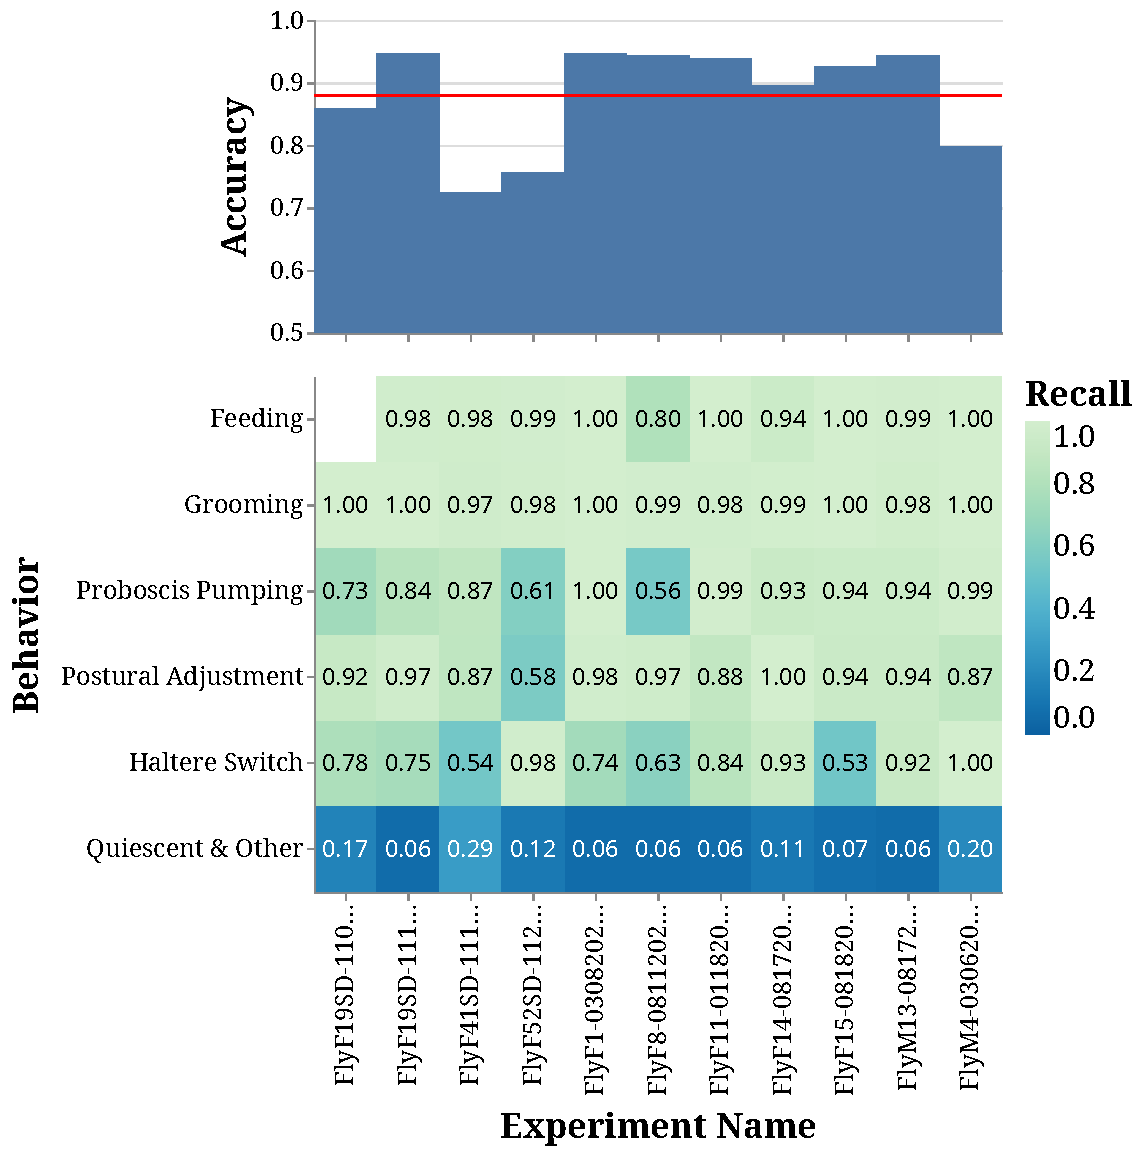
\includegraphics[width=\linewidth]{figures/OutliningPerformance-Supervised.pdf}
		\caption{Supervised detection.}
	\end{subfigure}%
	\hfill
	\begin{subfigure}[ht!]{0.495\linewidth}
		\centering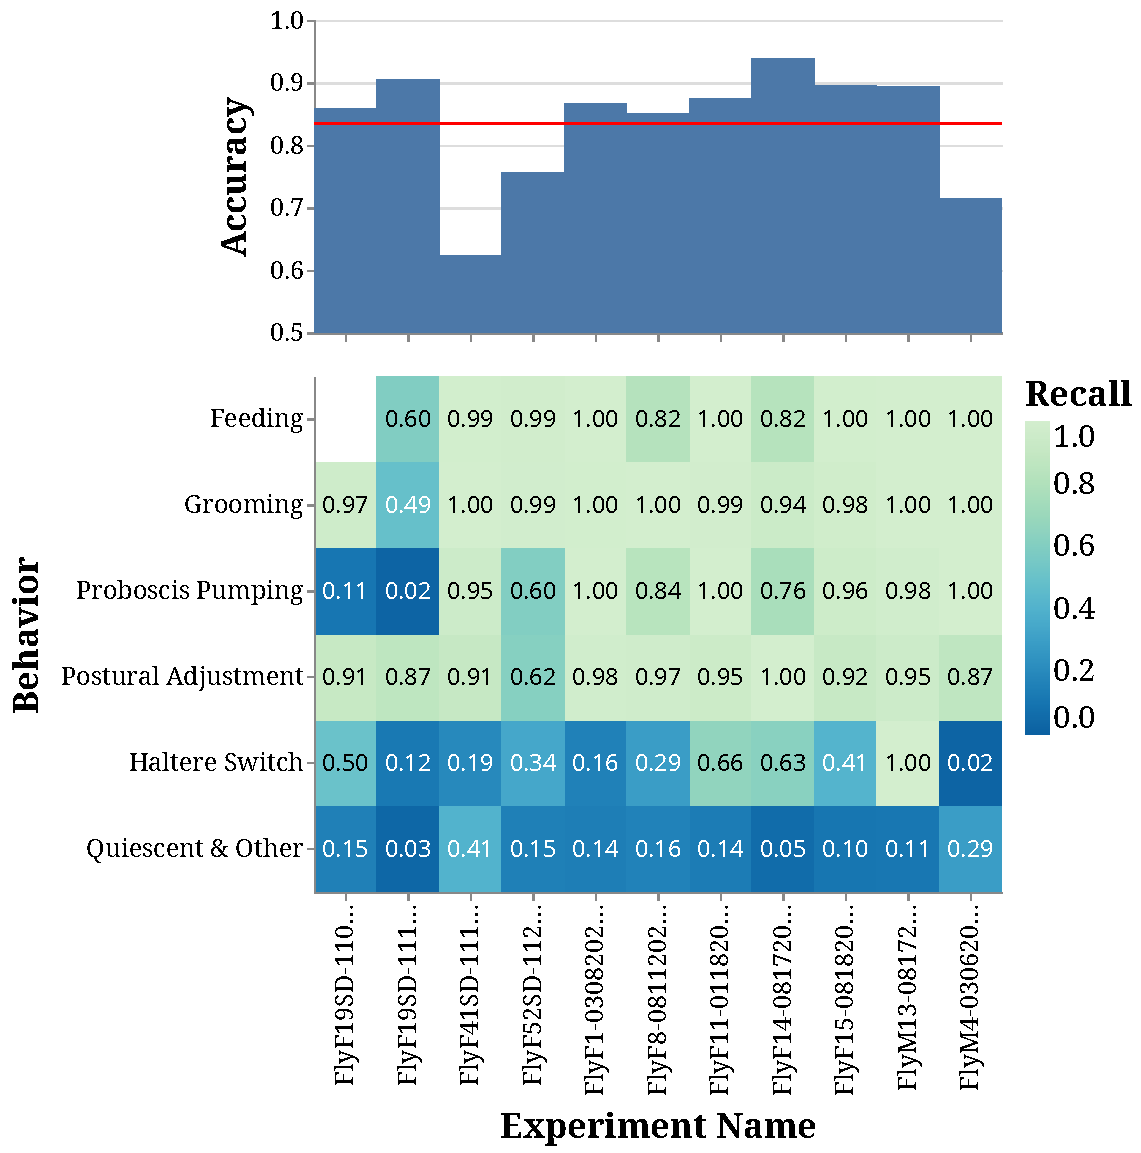
\includegraphics[width=\linewidth]{figures/OutliningPerformance-Unsupervised.pdf}
		\caption{Unsupervised detection.}
	\end{subfigure}%
	\caption[Performance summary of experiment outlining and micro-activity detection.]{Performance summary of experiment outlining and micro-activity detection.
		Red line indicates the macro average of accuracy scores achieved for each split.
		High recall scores are desired for behavioral categories, as opposed to quiescent frames.
		Supervised and unsupervised detections are given respectively in the left subfigure and in the right subfigure.}
\end{figure}

\begin{figure}[ht!]
	\centering
	\begin{subfigure}[ht!]{0.495\linewidth}
		\centering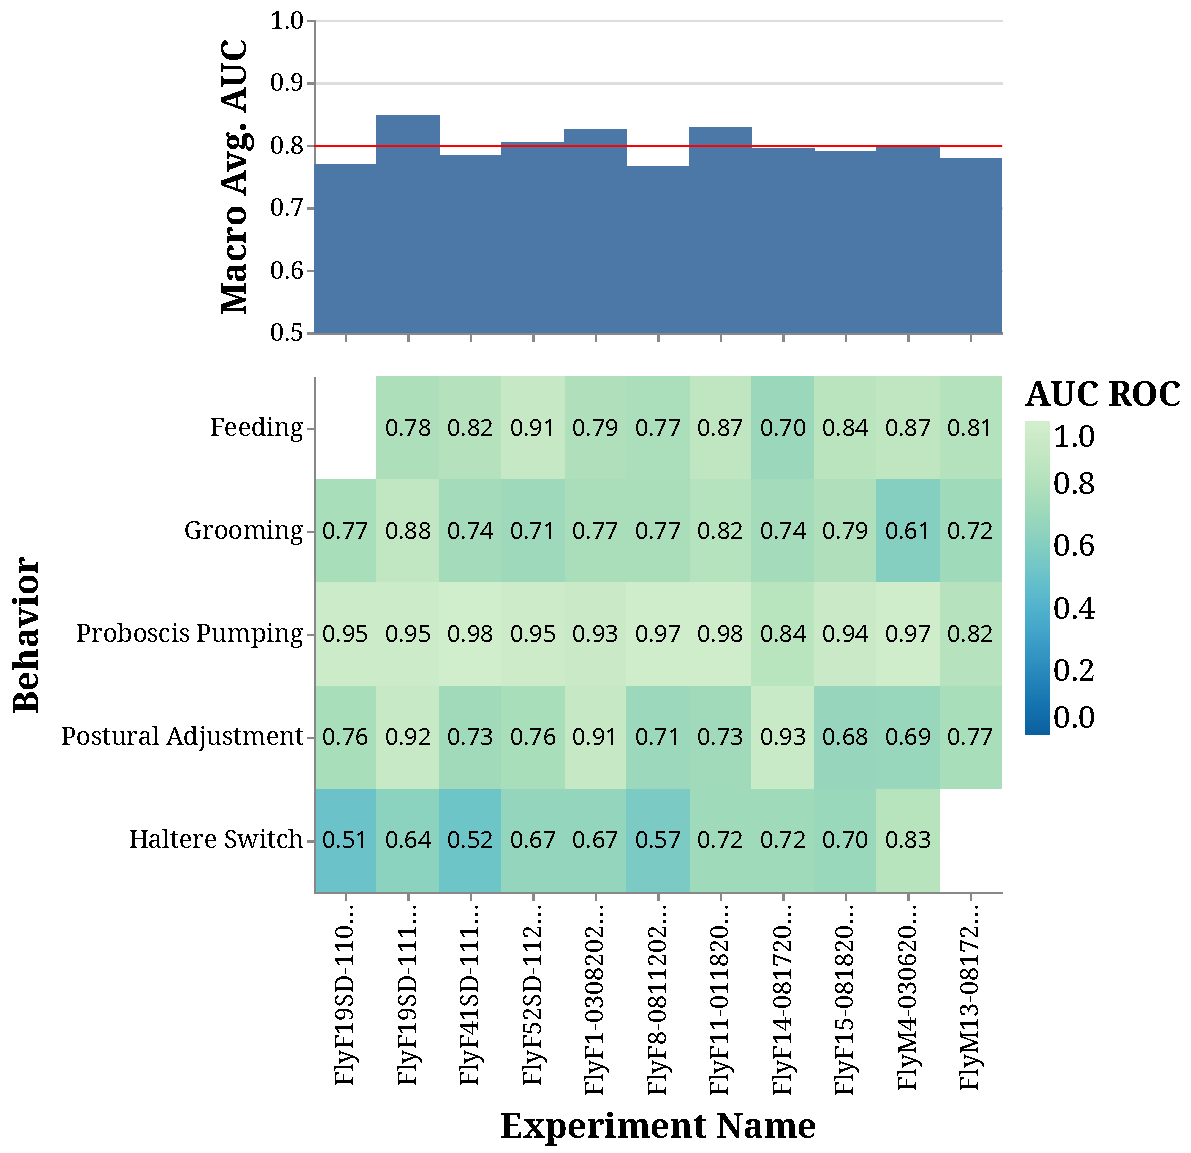
\includegraphics[width=\linewidth]{figures/AUC_ROC-DActfiltered.pdf}
		\caption{AUC scores for $\MicroActivity$ set. \label{figure:AUC-ROC-Act}}
	\end{subfigure}%
	\hfill
	\begin{subfigure}[ht!]{0.495\linewidth}
		\centering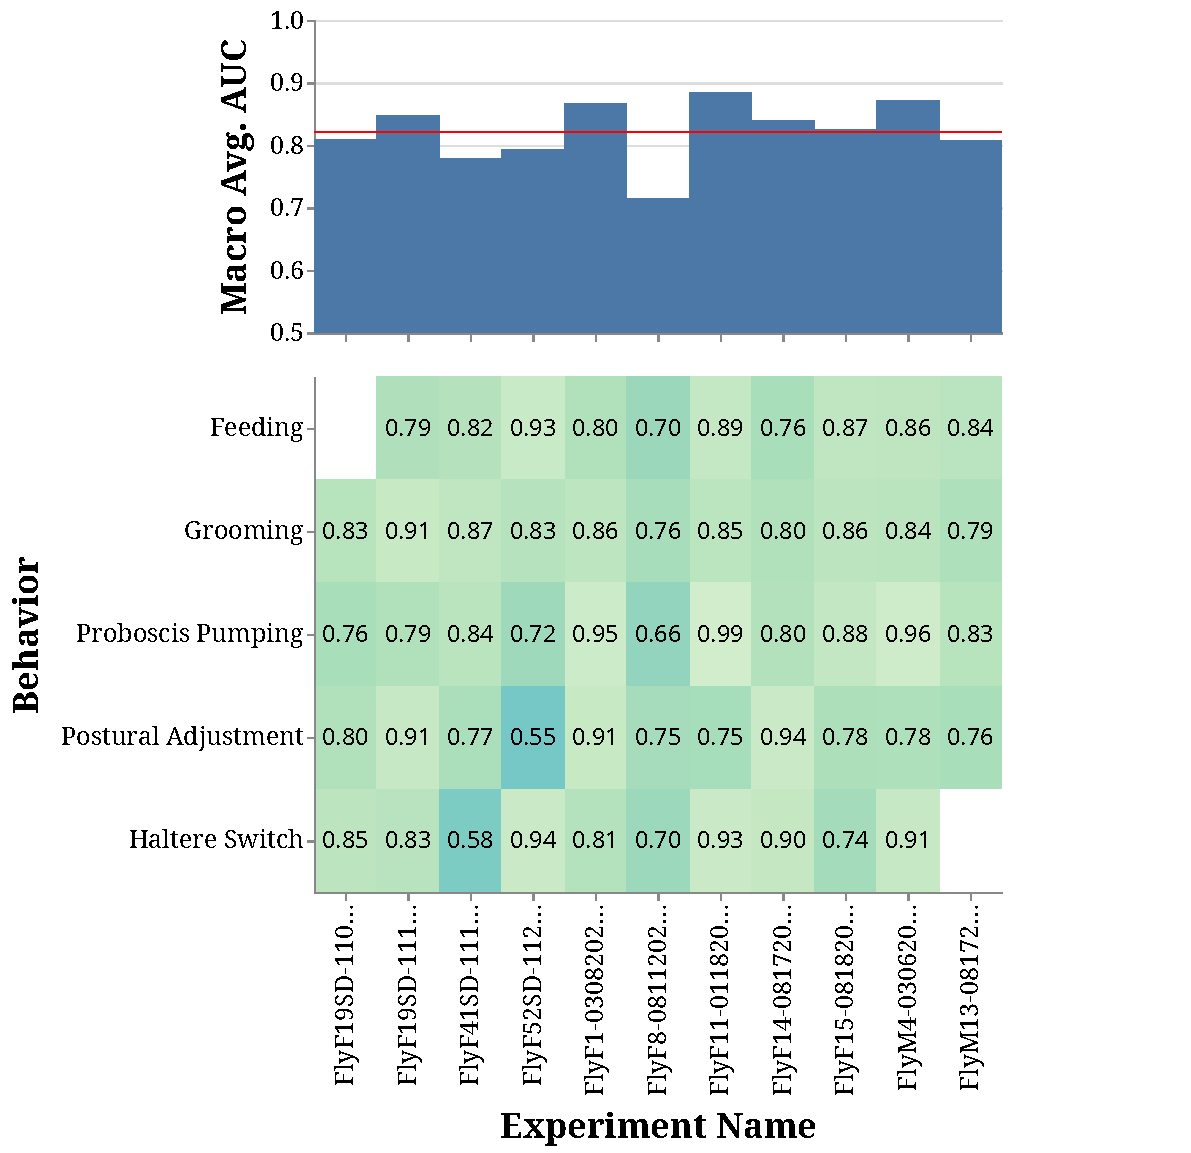
\includegraphics[width=\linewidth]{figures/AUC_ROC-DAnnfiltered.pdf}
		\caption{AUC scores for annotated frames. \label{figure:AUC-ROC-Ann}}
	\end{subfigure}%

	\begin{subfigure}[ht!]{0.95\linewidth}
		\centering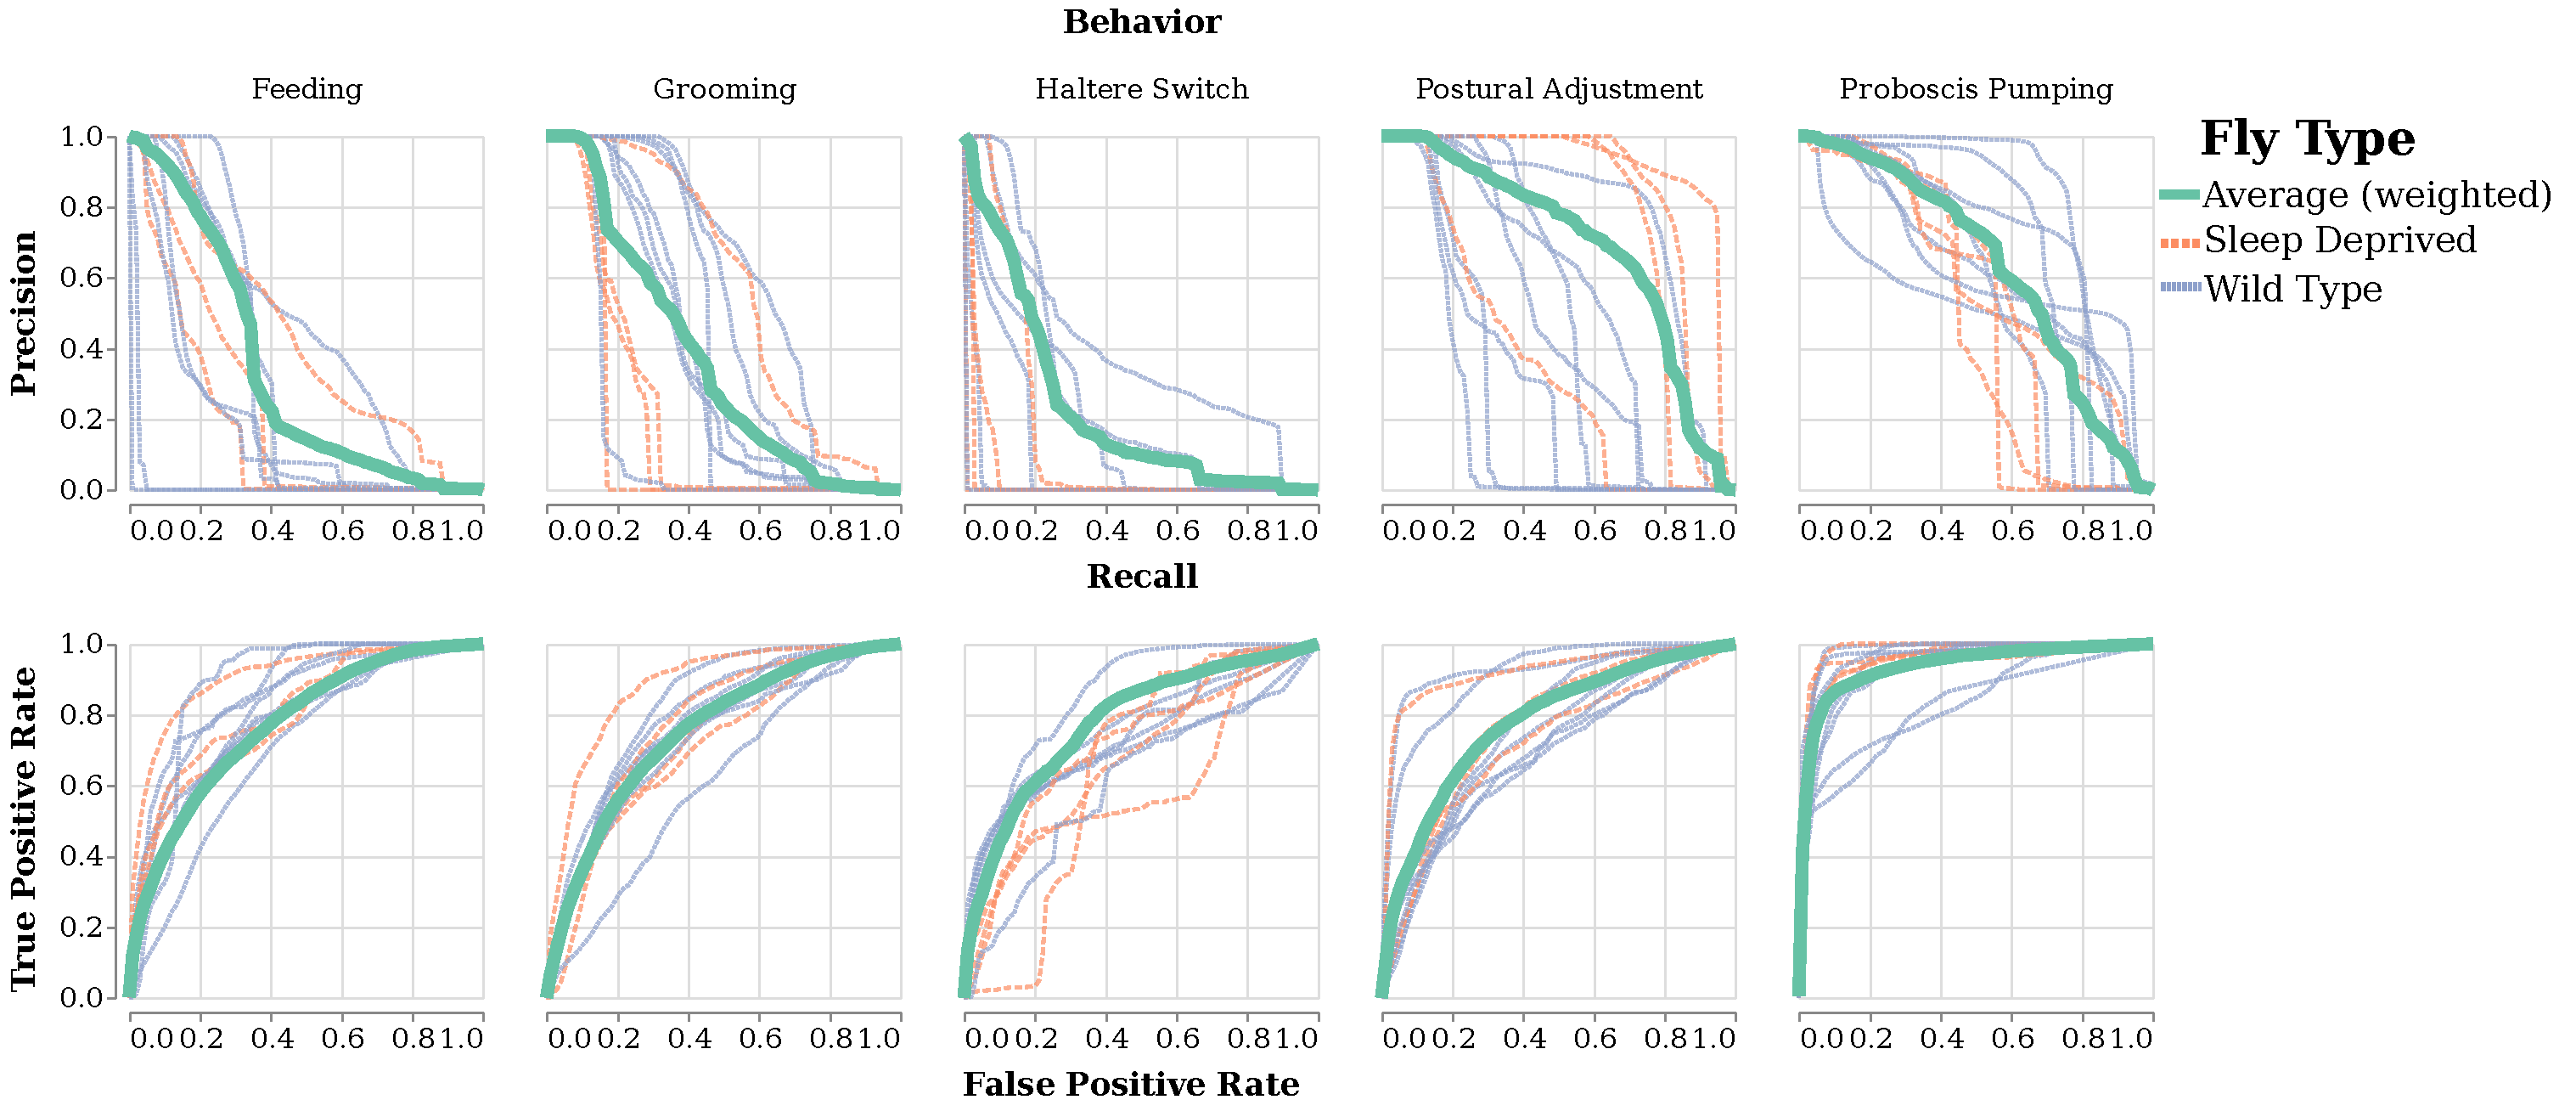
\includegraphics[width=\linewidth]{figures/PRC_ROC-DActfiltered.pdf}
		\caption{ROC and precision-recall curves for frames detected as micro-activity. \label{figure:ROC-PRC-Act}}
	\end{subfigure}%

	\begin{subfigure}[ht!]{0.95\linewidth}
		\centering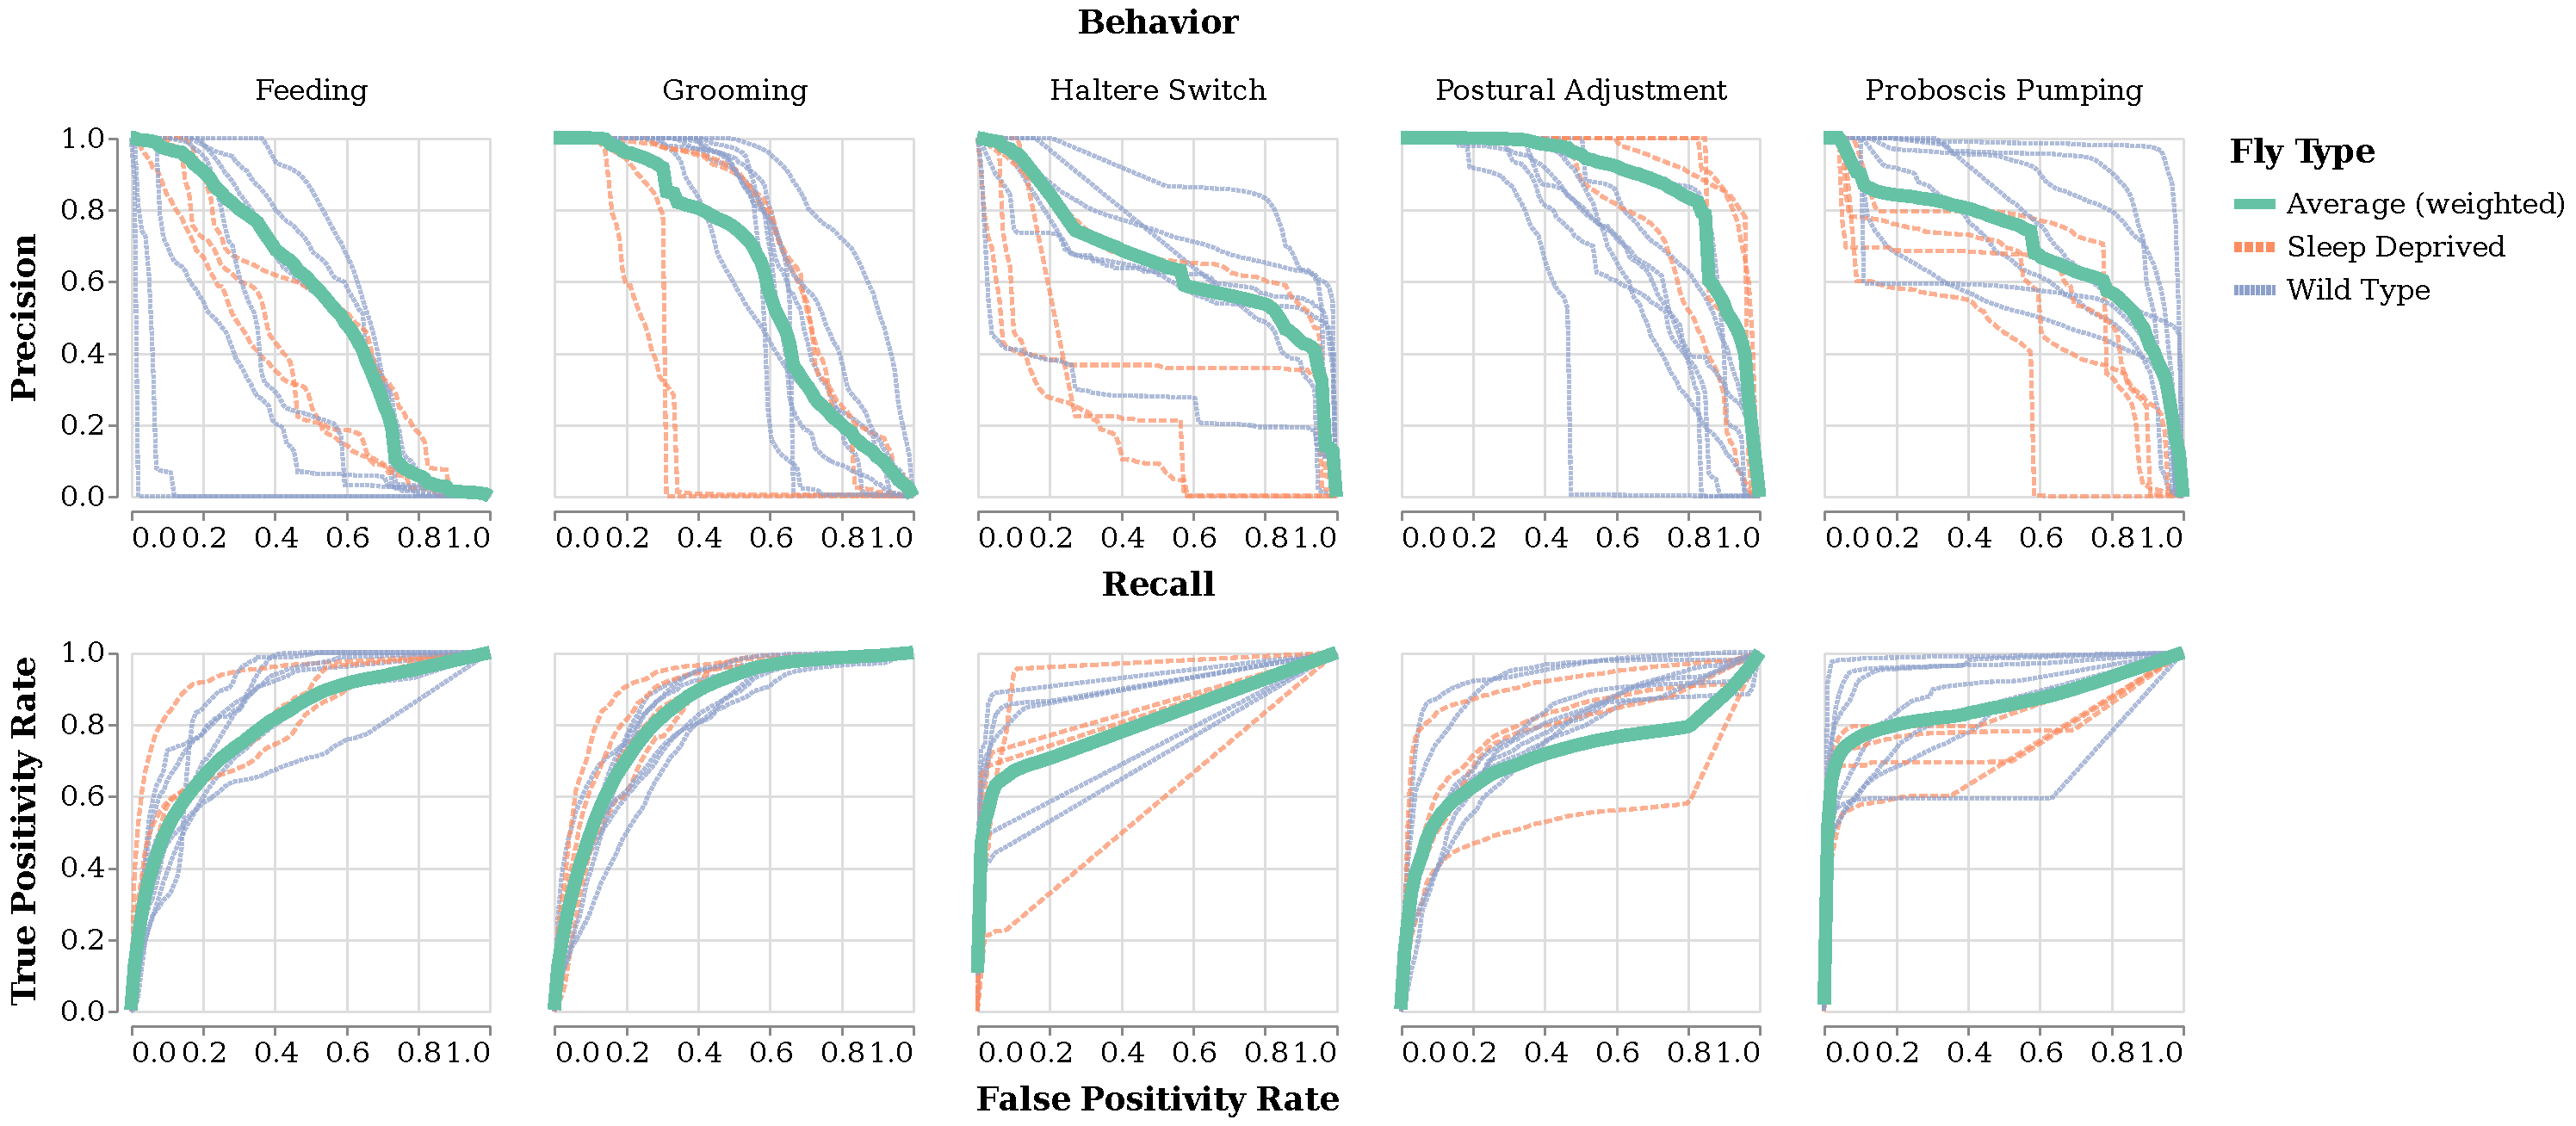
\includegraphics[width=\linewidth]{figures/PRC_ROC-DAnnfiltered.pdf}
		\caption{ROC and precision-recall curves for annotated frames. \label{figure:ROC-PRC-Ann}}
	\end{subfigure}%
	\caption[Performance summary of behavior mapping demonstrated using receiver operating characteristic curve, precision-recall curve, and area under curve scores.
	]{Performance summary of behavior mapping demonstrated using receiver operating characteristic curve, precision-recall curve, and area under curve scores.
		The red line indicates the macro average of AUC scores for each split.
		Weighted average of ROC and precision-recall curves computed by interpolation.
		Scores and curves for both frames estimated as micro-activity and annotated frames are given respectively in Figures~\ref{figure:AUC-ROC-Act}, ~\ref{figure:ROC-PRC-Act} and in Figures~\ref{figure:AUC-ROC-Ann}, ~\ref{figure:ROC-PRC-Ann}.}
\end{figure}

\begin{figure}[ht!]
	\centering
	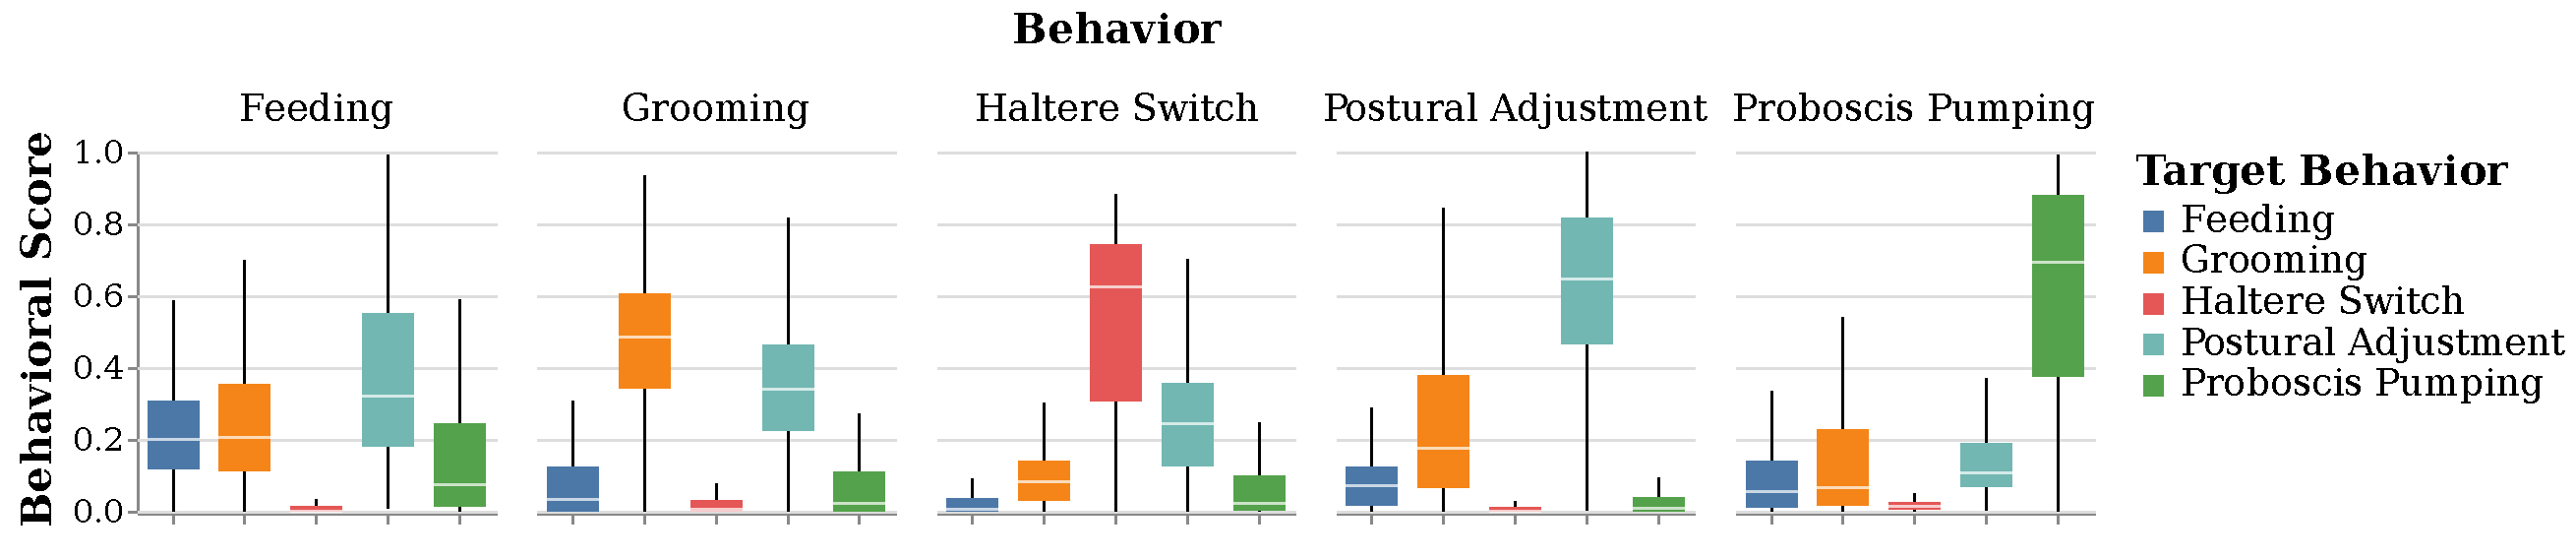
\includegraphics[width=\linewidth]{figures/BehavioralScoresDistributions_perBehavior.pdf}
	\caption[Distributions of behavioral score values of each behavioral category for all splits.]{Distributions of behavioral score values of each behavioral category for all splits.
		Each box-plot column demonstrates the behavioral score distributions of target behaviors for the corresponding annotation.}
\end{figure}

\begin{figure}[ht!]
	\centering
	\begin{subfigure}[h]{0.55\linewidth}
		\centering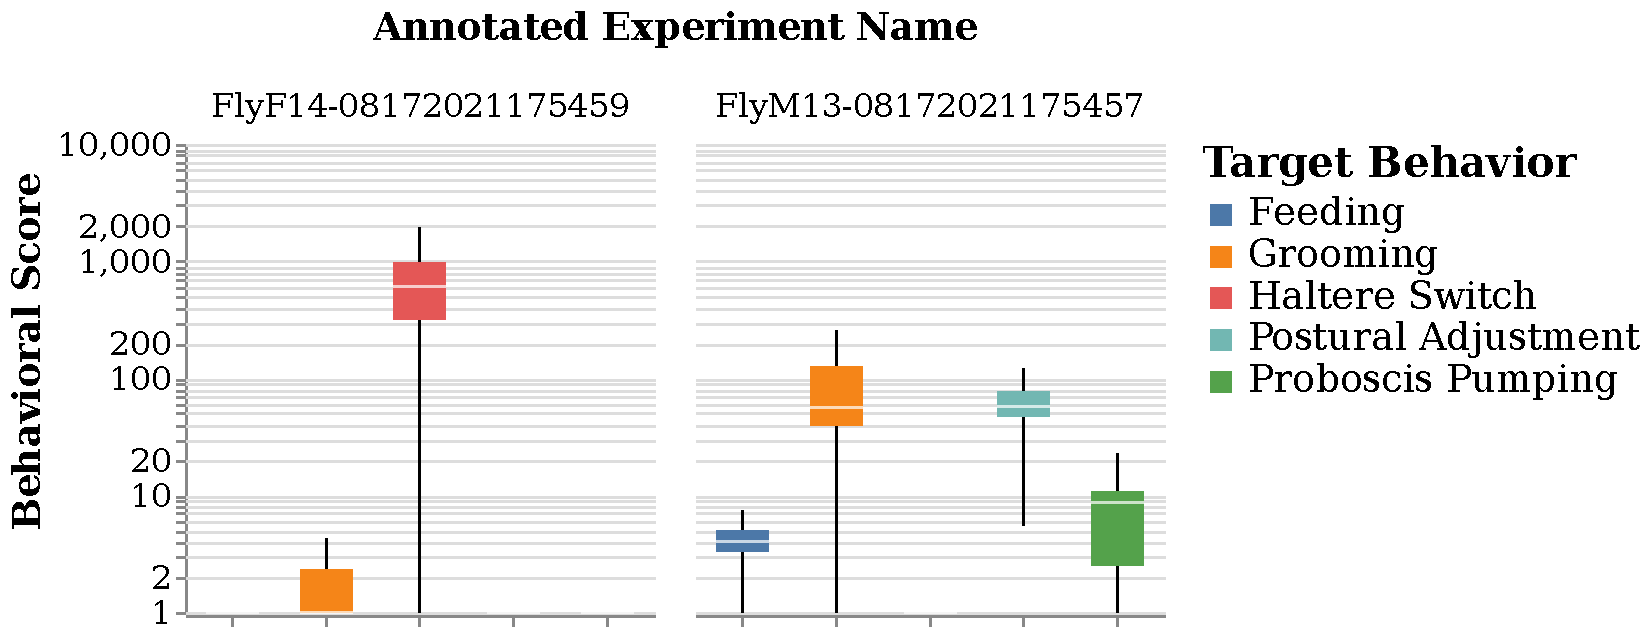
\includegraphics[width=\linewidth]{figures/BehavioralScores-RepertoireDifference.pdf}
		\caption{Behavioral score values.}
	\end{subfigure}%
	\centering
	\begin{subfigure}[h]{0.45\linewidth}
		\centering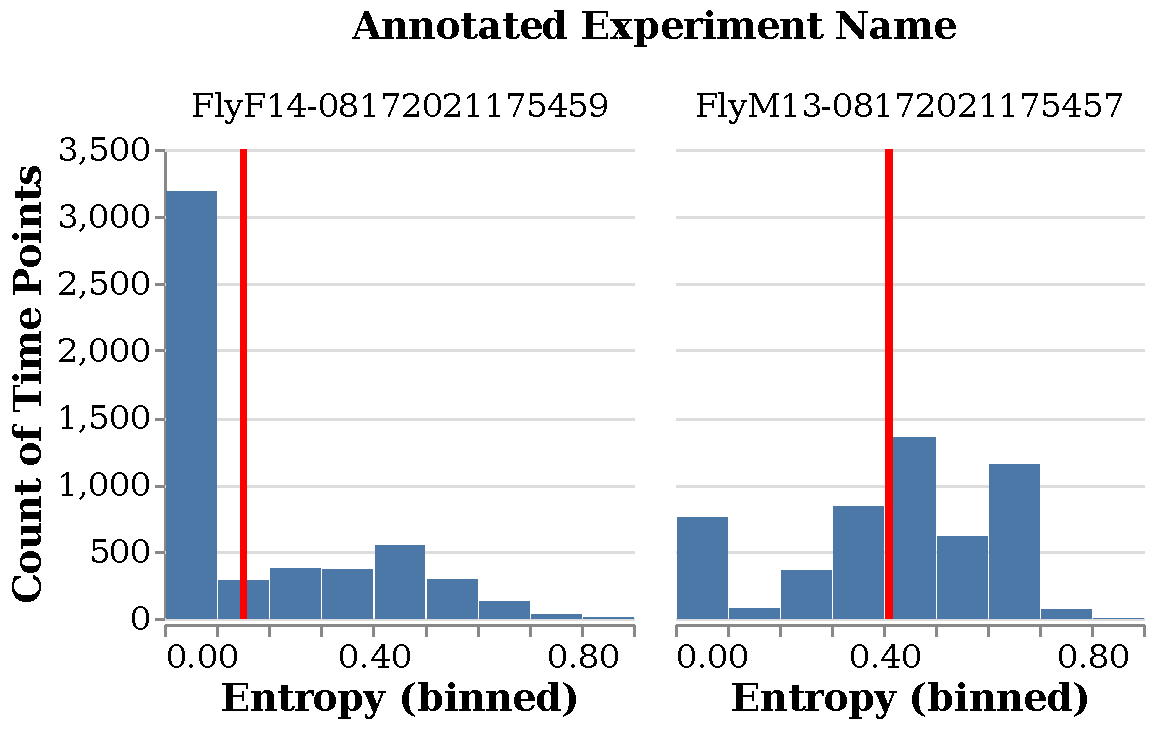
\includegraphics[width=\linewidth]{figures/Entropy-RepertoireDifference.pdf}
		\caption{Entropy values, red line is the mean.}
	\end{subfigure}%
	\caption[Histogram of entropy values and box-plot of the behavioral scores computed using one unannotated and two annotated experiments with varying behavioral repertoires.]{Histogram of entropy values and box-plot of behavioral scores computed using one unannotated and two annotated experiments with varying behavioral repertoires.
		Here behavioral repertoire of FlyF1-03082020 is predicted separately with two different annotated experiments, namely FlyF14-08172021 and FlyM13-08172021.
		Behavioral scores and entropy values are computed for the haltere switch behavior.
		The latter one lacks the haltere switch behavior, and as a result behavioral scores tend to have higher entropy.
		Results demonstrates ability of the proposed pipeline to detect and discover new unannotated behavioral categories using behavioral scores.}
\end{figure}

\section{Analyzing Behavioral Repertoire}\label{section:analyzing-behavioral-repertoire}

\begin{figure}[ht!]
	\centering
	\begin{subfigure}[ht!]{0.95\linewidth}
		\centering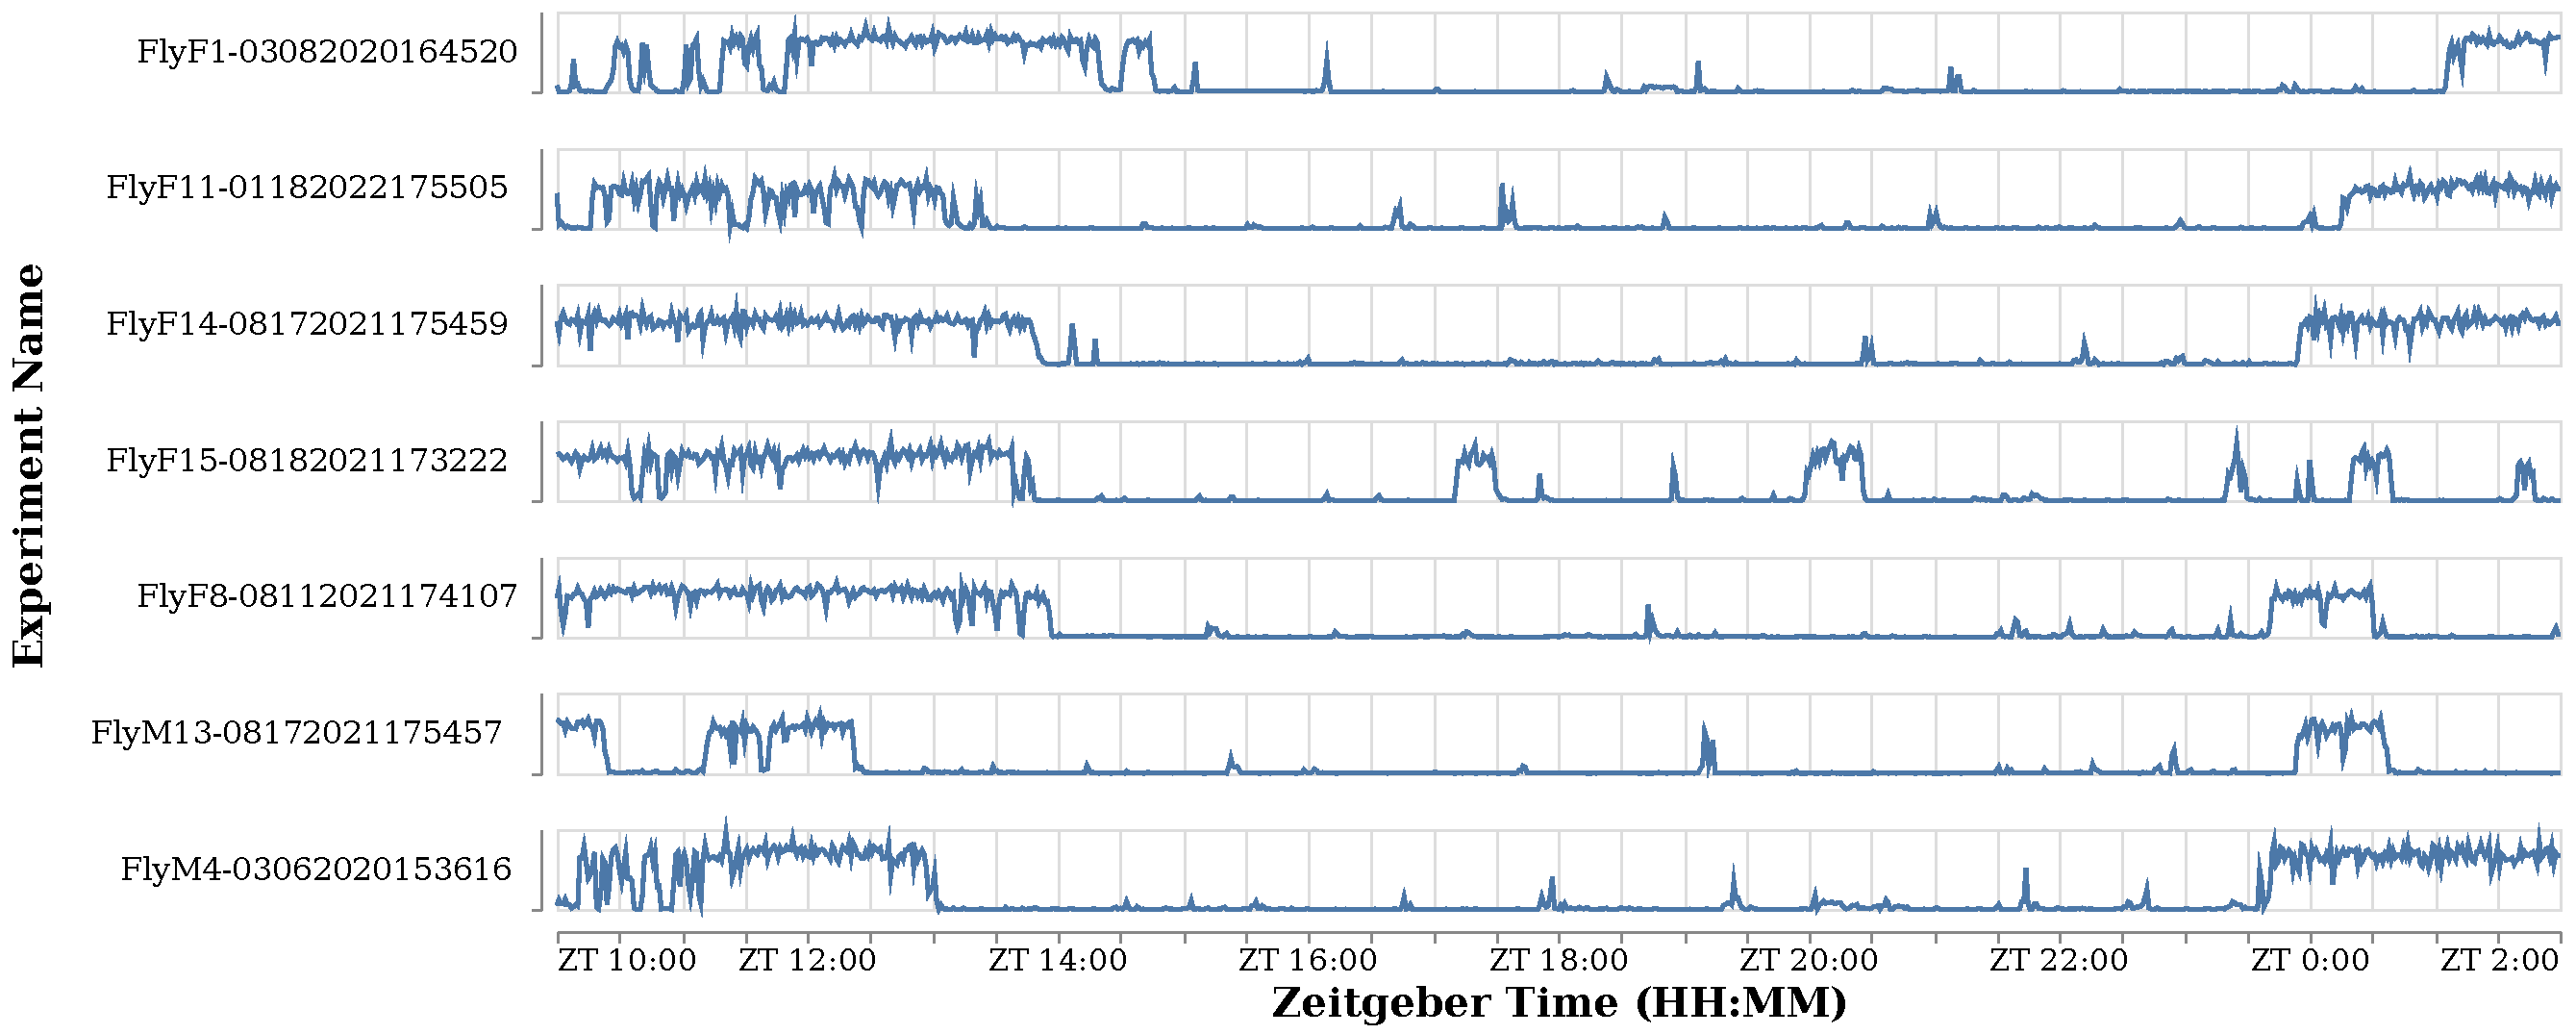
\includegraphics[width=\linewidth]{figures/Velocity-WT-1T.pdf}
		\caption{Wild type.}
	\end{subfigure}%

	\begin{subfigure}[ht!]{0.95\linewidth}
		\centering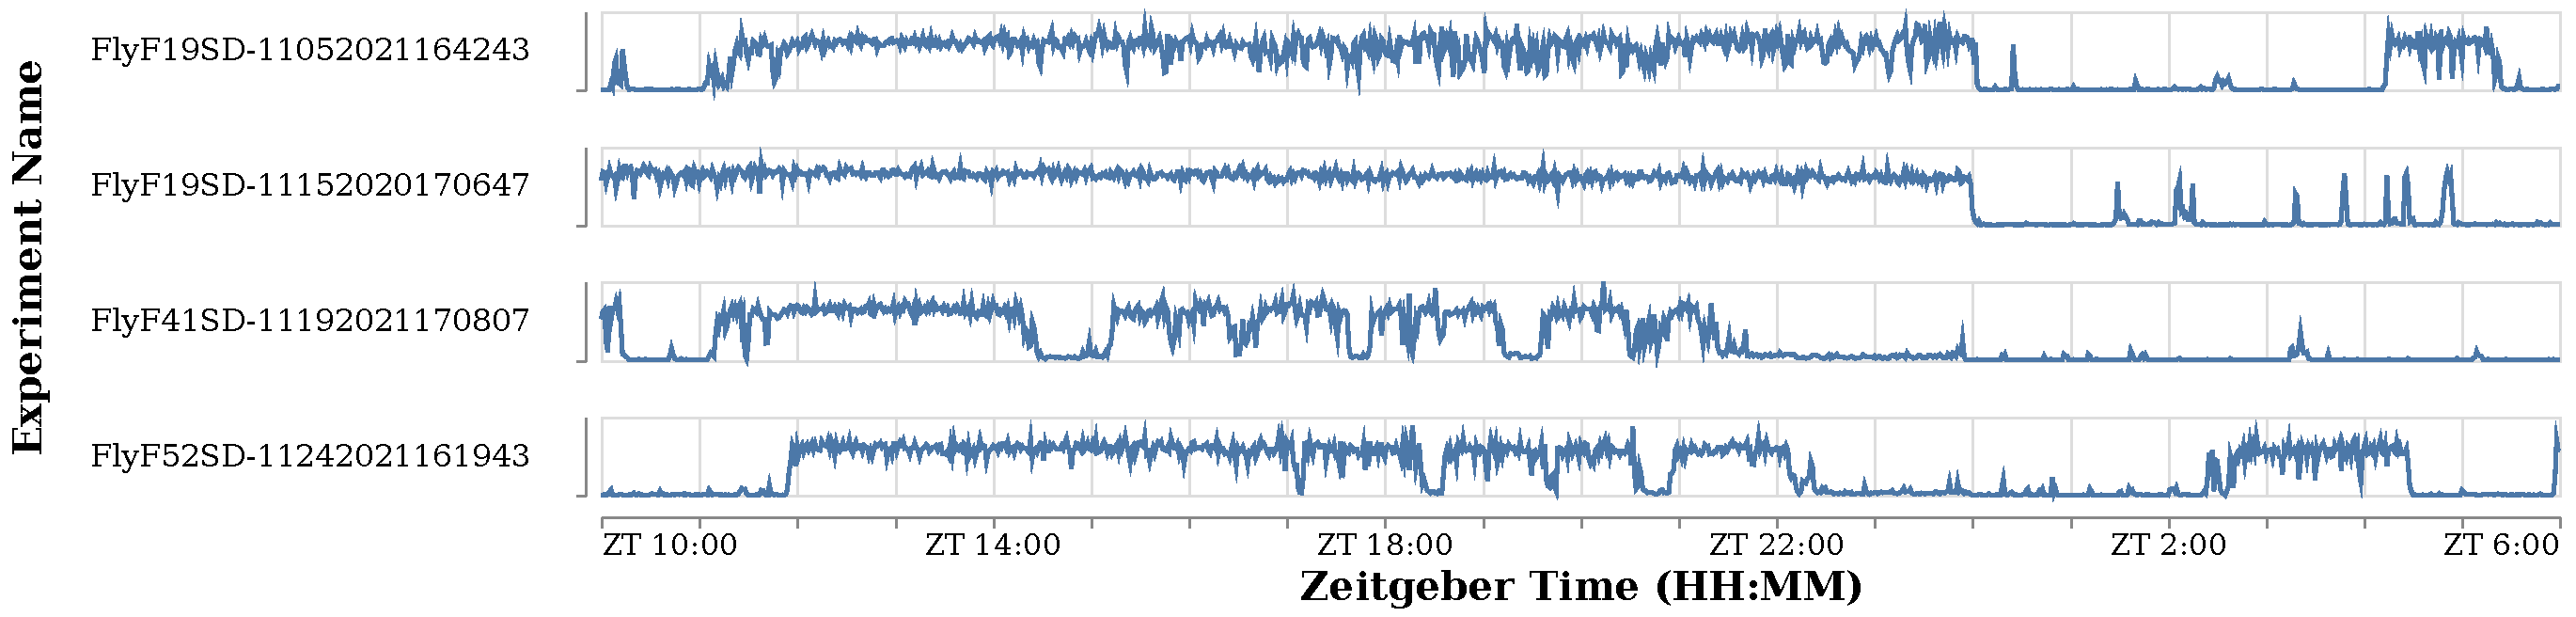
\includegraphics[width=\linewidth]{figures/Velocity-SD-1T.pdf}
		\caption{Sleep deprived.}
	\end{subfigure}%
	\caption[Overall displacement values over entire experiments.]{Overall displacement values over entire experiments.
		Displacement of the body reveals long dormancy and sleep epochs, and macro-activities.
		Displacement values are computed as described in Equation~\ref{equation:displacement}, and smoothed with a rolling mean of 1 minute window.}
\end{figure}

\begin{figure}[ht!]
	\centering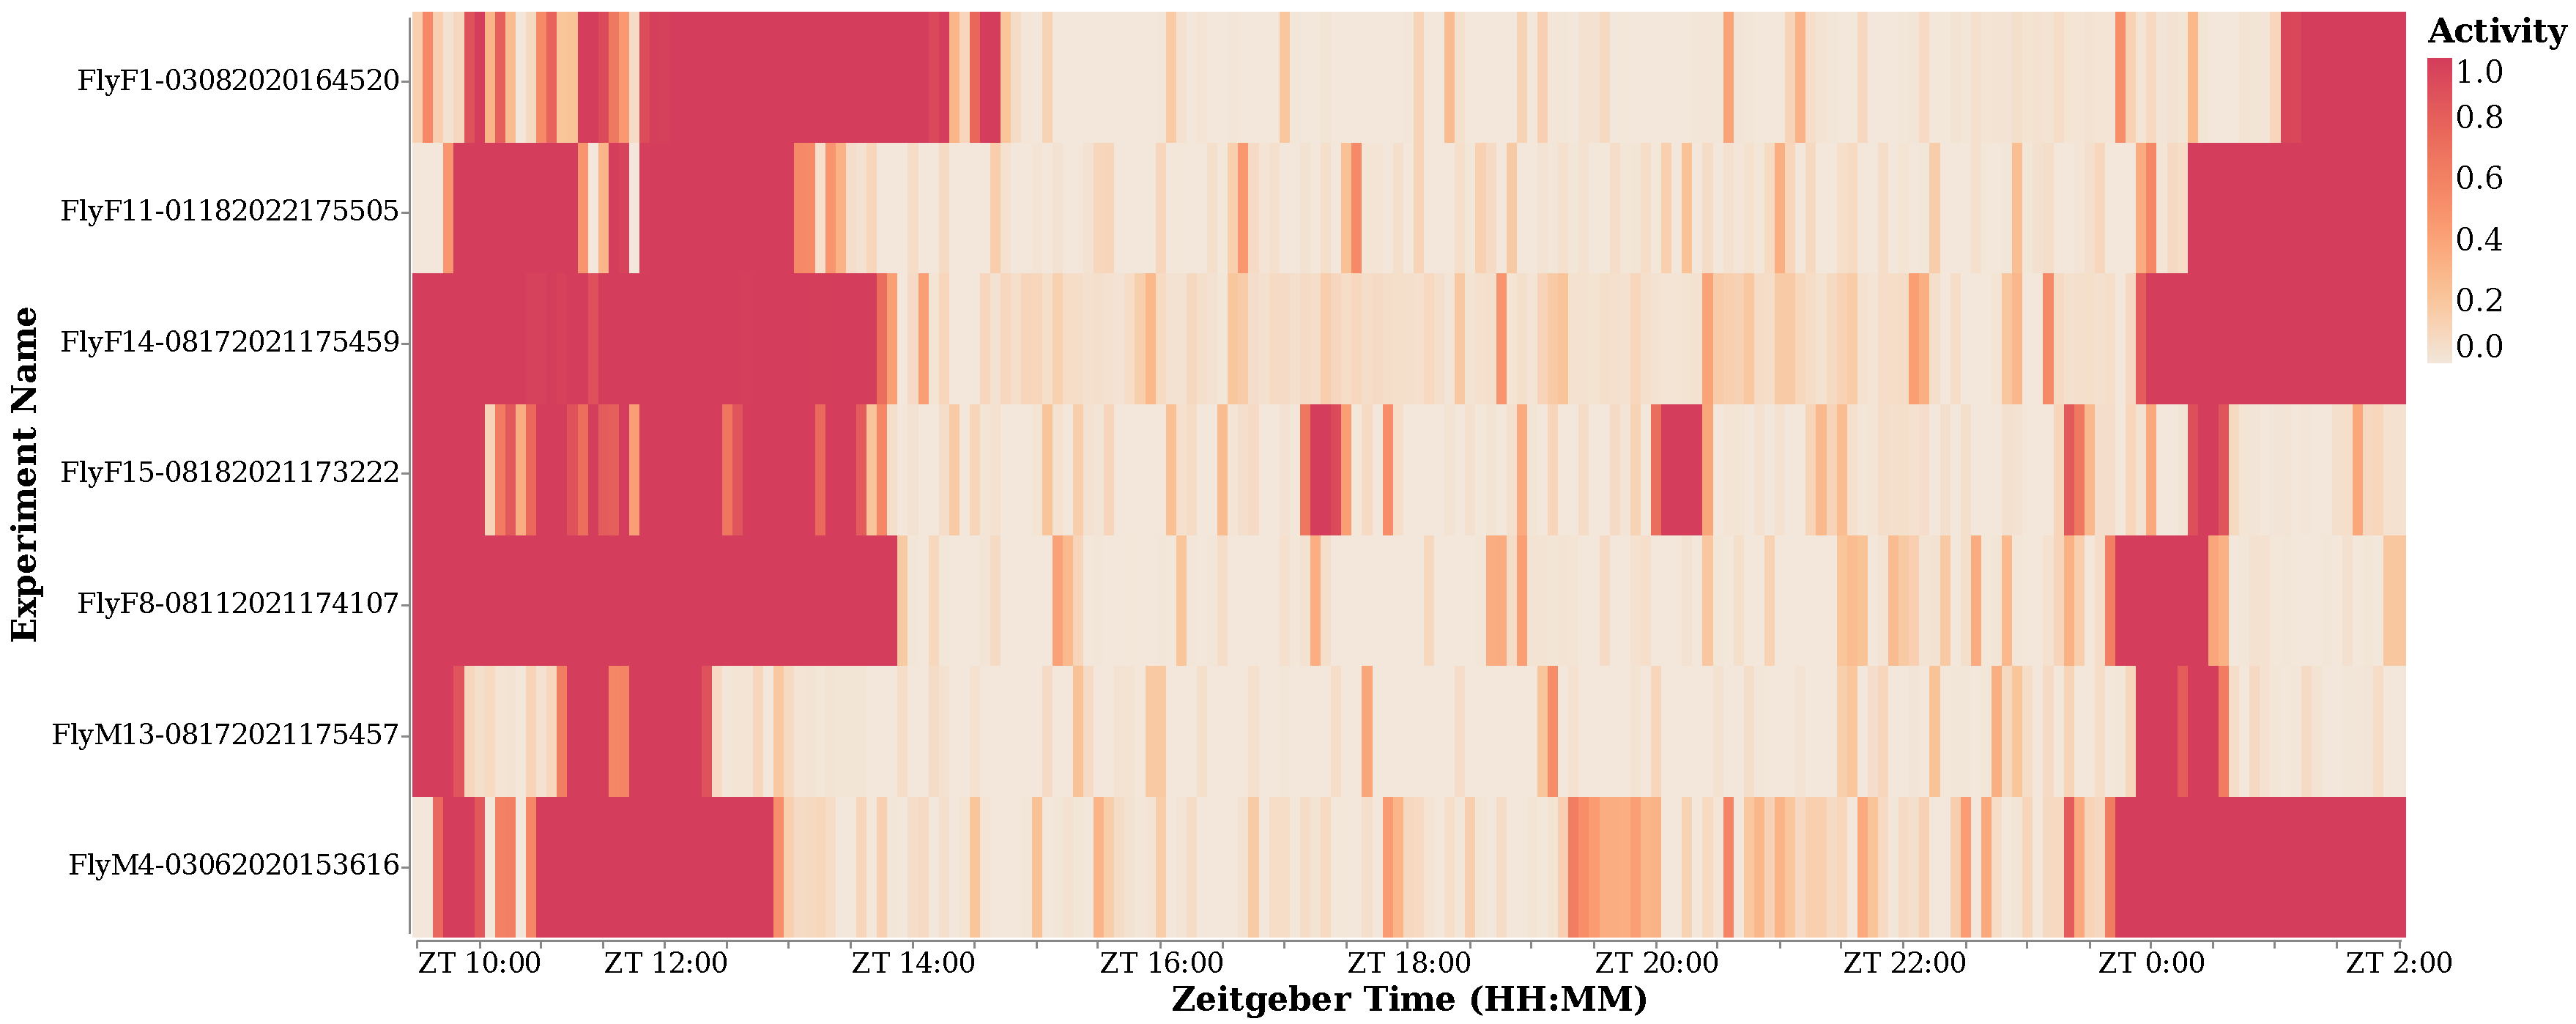
\includegraphics[width=\linewidth]{figures/ActivityBinned-Ann-WT-5T.pdf}
	\caption[Binned temporal heatmap of activities.]{Binned temporal heatmap of activities.
		Each bin is 5 minutes, corresponding to 900 frames.
		Activity value is computed as the ratio of the number of annotated frames and total number of frames in that bin.}
\end{figure}

\begin{figure}[ht!]
	\centering
	\begin{subfigure}[ht!]{0.95\linewidth}
		\centering
		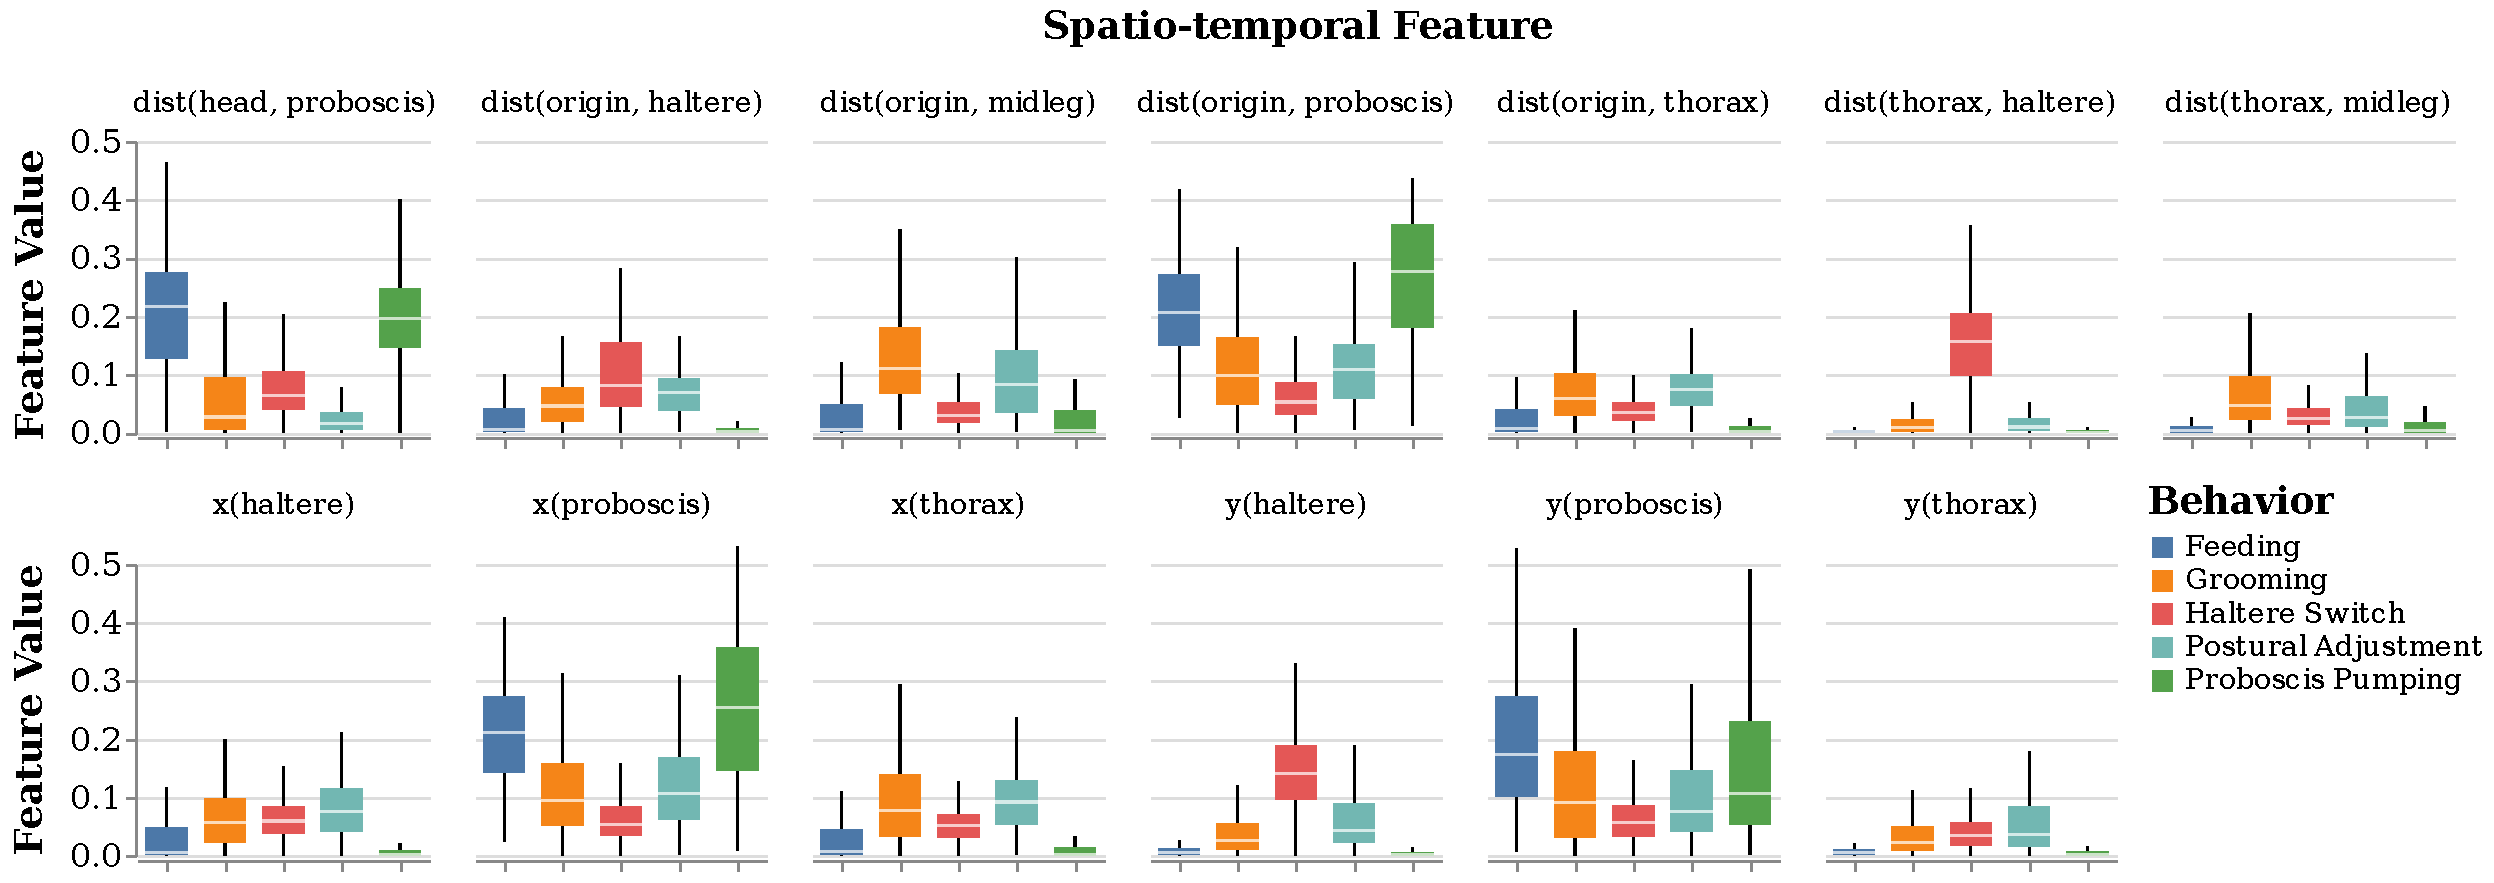
\includegraphics[width=\linewidth]{figures/FeatureDistributions_perBehavior-Ann.pdf}
		\caption{Summation of all frequency channels of behavioral representation value for each spatio-temporal feature.}
	\end{subfigure}%

	\centering
	\begin{subfigure}[ht!]{0.95\linewidth}
		\centering
		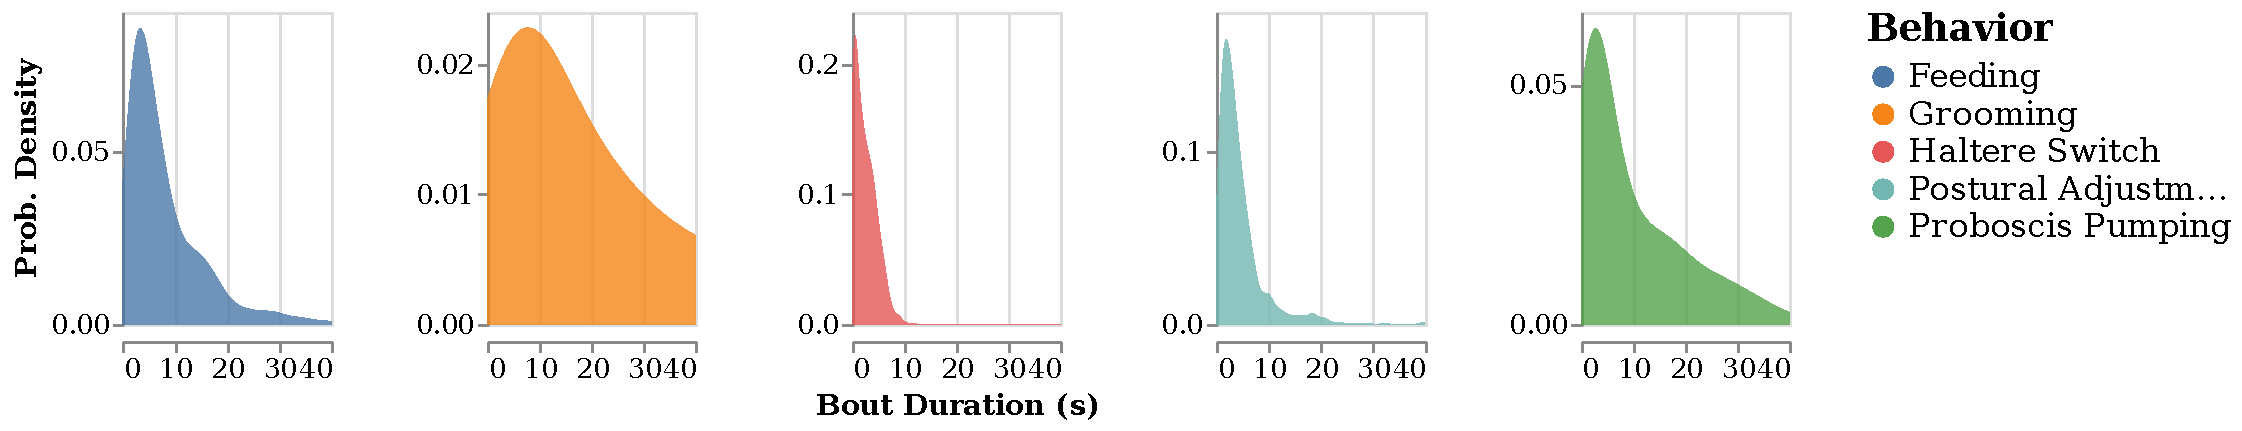
\includegraphics[width=\linewidth]{figures/BoutDurationDistributions-Ann.pdf}
		\caption{Kernel density estimations of bout durations for each behavioral category. Variance of bout durations within and across behavioral categories demonstrates the rich behavioral repertoire.}
	\end{subfigure}%

	\centering
	\begin{subfigure}[ht!]{0.95\linewidth}
		\centering
		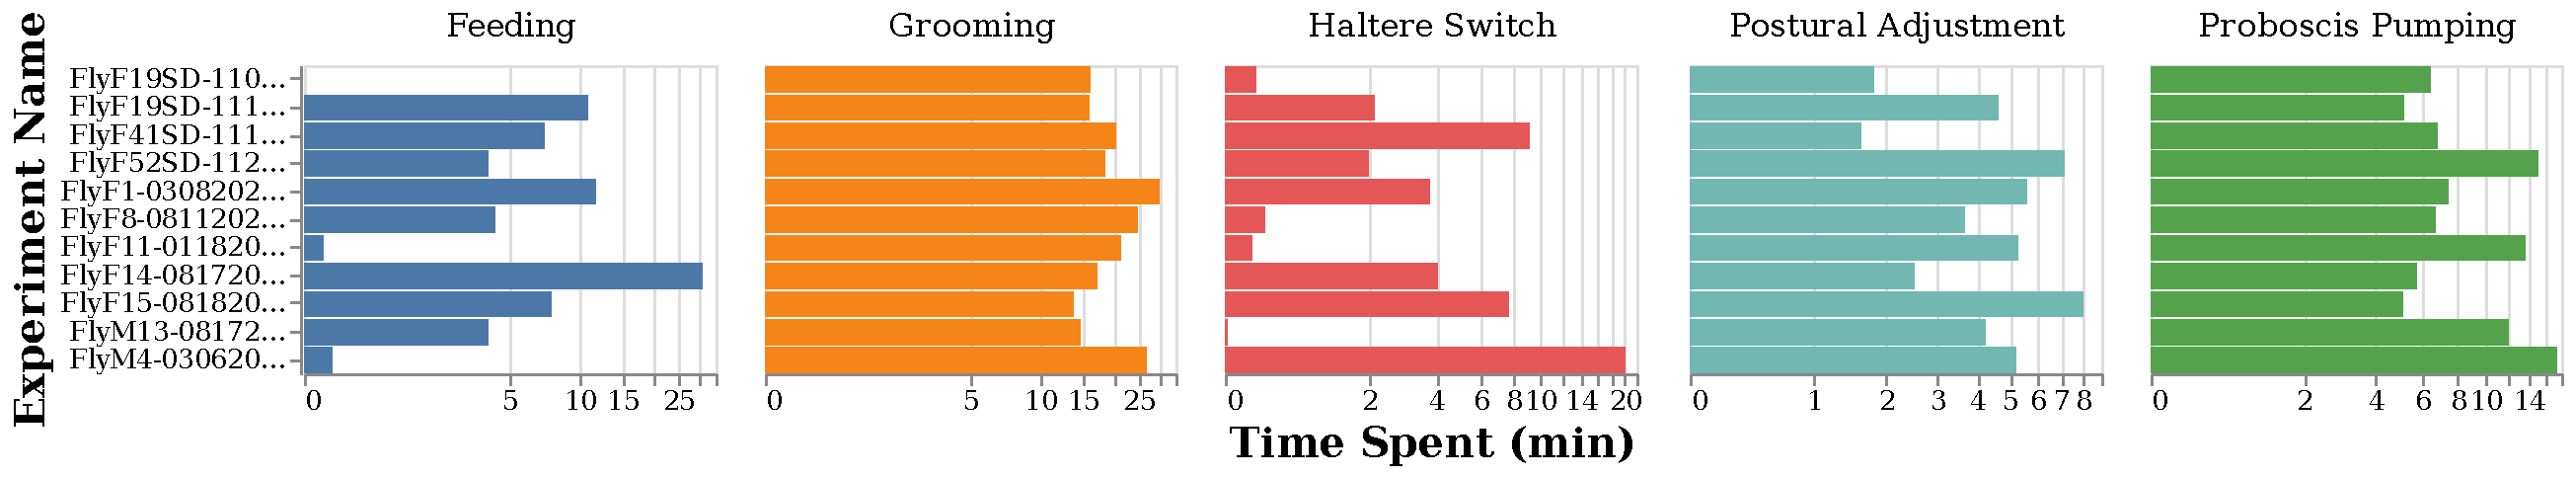
\includegraphics[width=\linewidth]{figures/TimeSpent-perBehavior-Ann.pdf}
		\caption{Time spent with each behavioral category for all experiments.}
	\end{subfigure}%
	\caption{Summary of behavioral repertoires of different fly, demonstrated using both spatial and temporal characteristics.}
\end{figure}

\begin{figure}[ht!]
	\centering
	\begin{subfigure}[ht!]{0.975\linewidth}
		\centering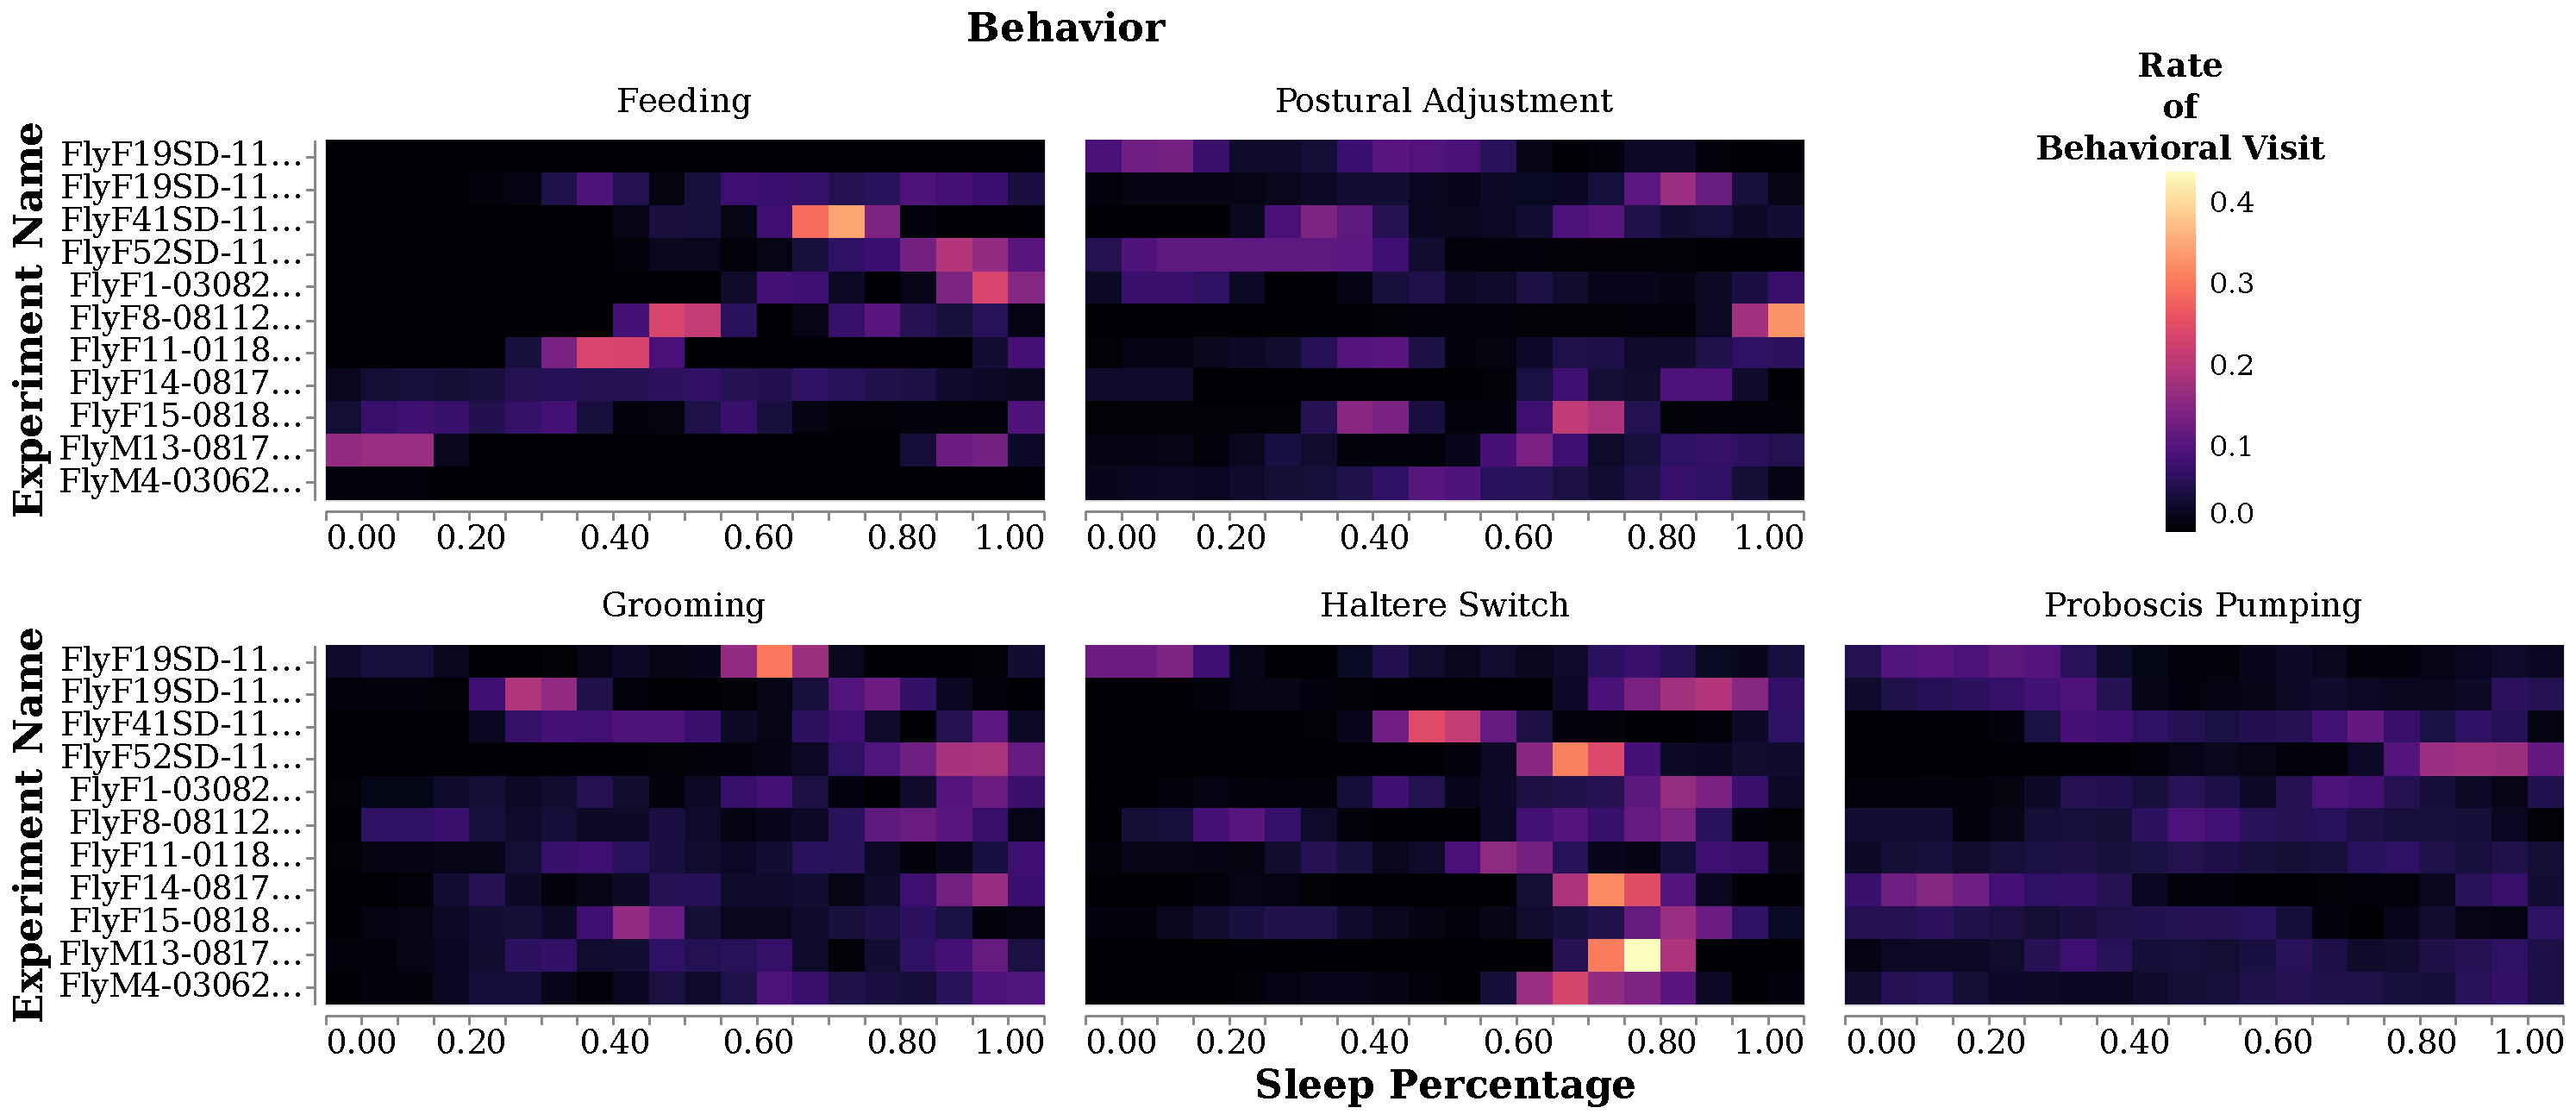
\includegraphics[width=\linewidth]{figures/Heatmap_BehavioralUsage-Ann.pdf}
		\caption{}
	\end{subfigure}%

	\centering
	\begin{subfigure}[ht!]{0.975\linewidth}
		\centering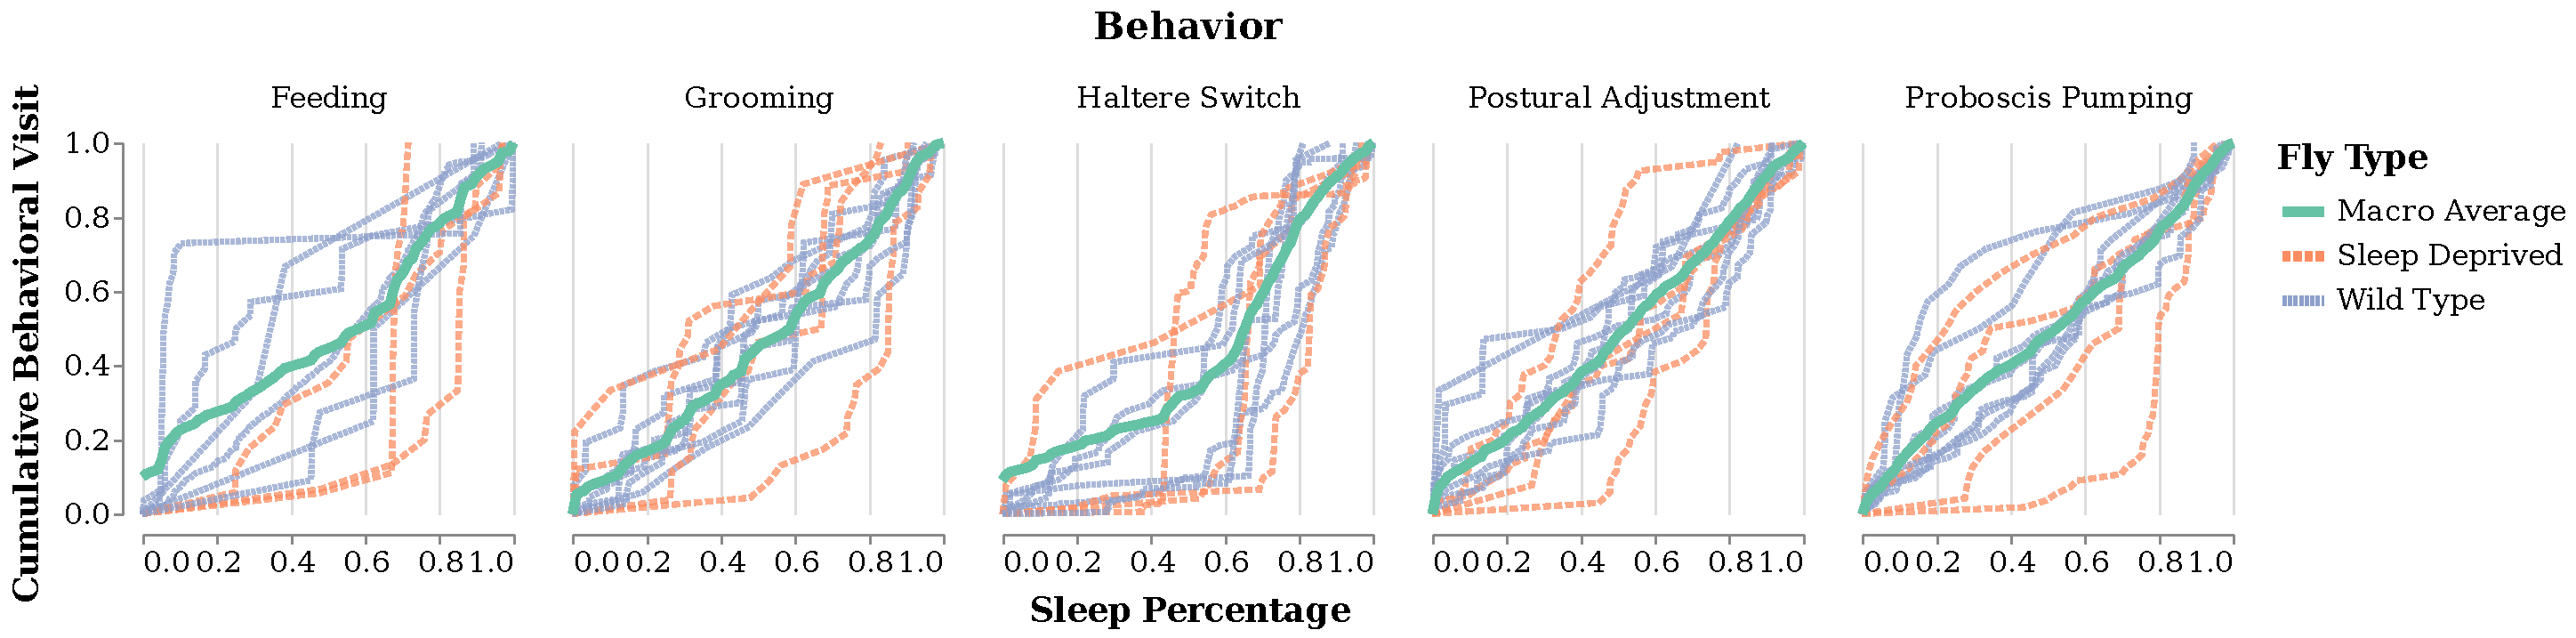
\includegraphics[width=\linewidth]{figures/CumulativeLine_BehavioralUsage-Ann.pdf}
		\caption{}
	\end{subfigure}%

	\centering
	\begin{subfigure}[ht!]{0.825\linewidth}
		\centering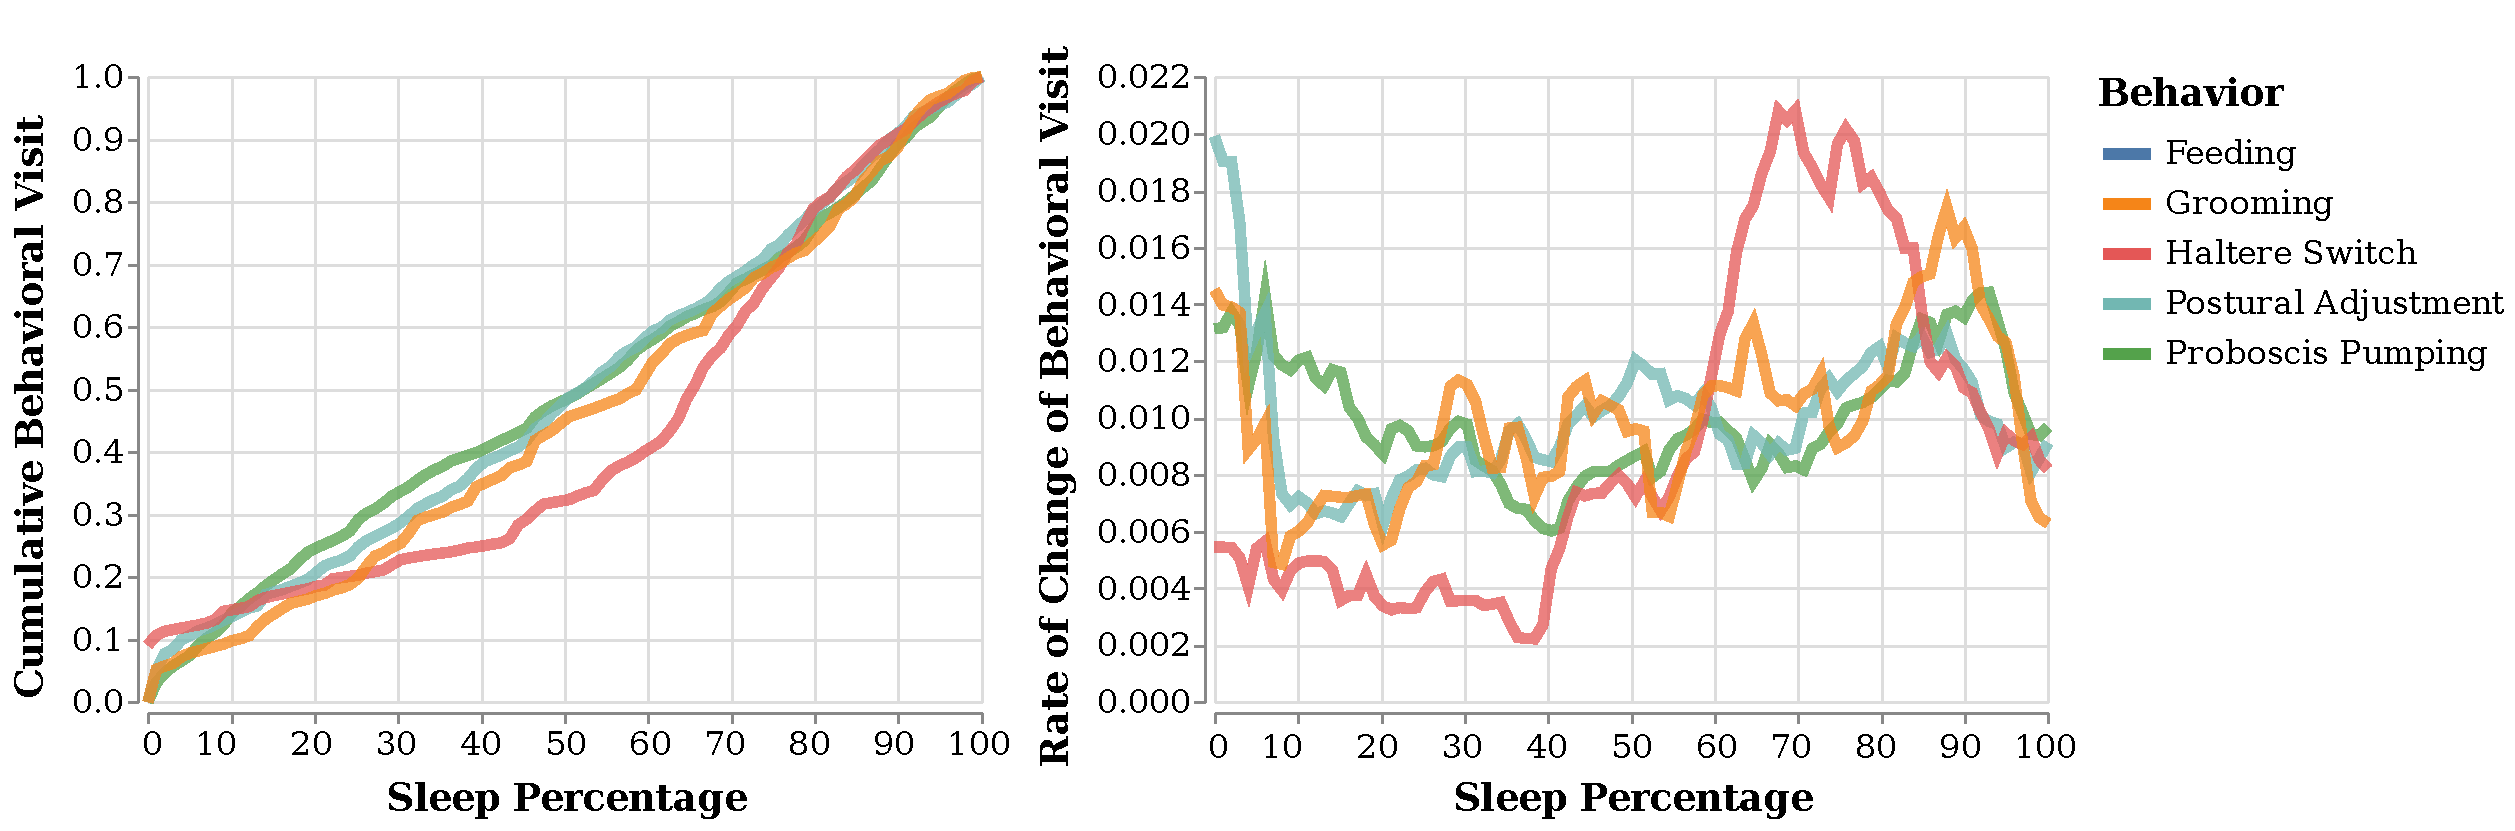
\includegraphics[width=\linewidth]{figures/MeanCumRofC_BehavioralUsage-Ann.pdf}
		\caption{}
	\end{subfigure}%

	\centering
	\begin{subfigure}[b]{0.45\linewidth}
		\centering
		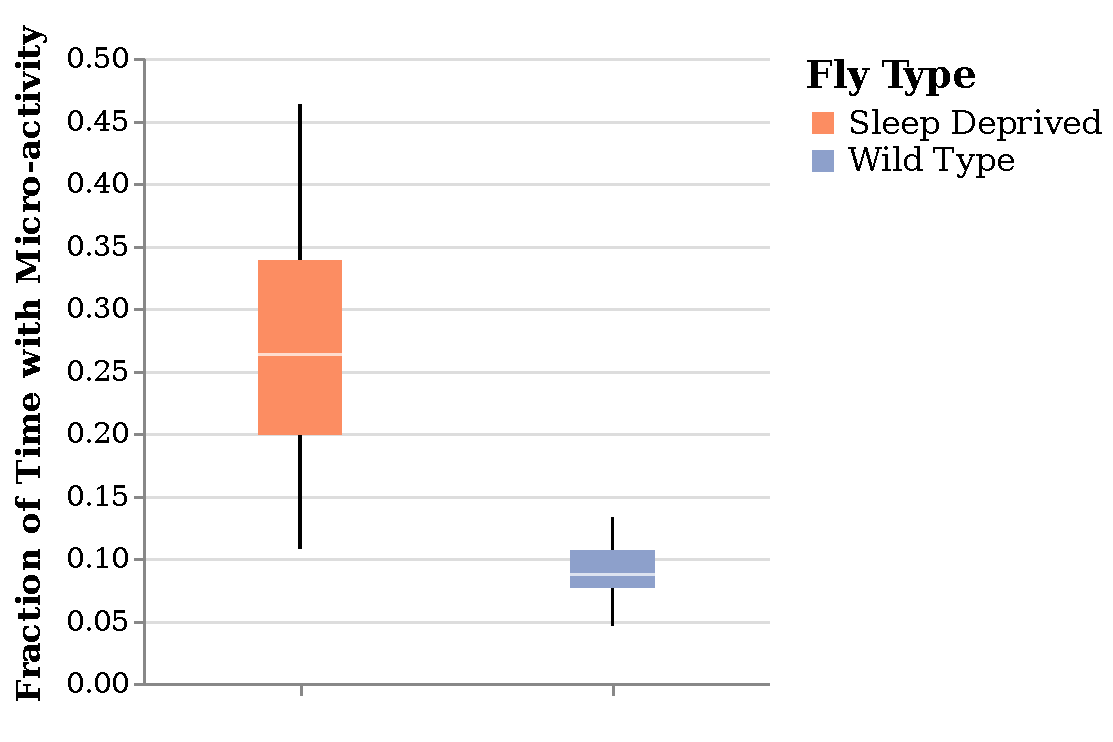
\includegraphics[width=\linewidth]{figures/FractionTime-Microactivity.pdf}
		\caption{Fraction of time spent with micro-activities in dormant epochs, comparing wild type experiments and sleep deprived experiments.}
	\end{subfigure}%

\end{figure}
